\documentclass[11pt,a4paper]{article}

\usepackage[a4paper,margin=2.5cm]{geometry}
\usepackage{amsmath}
\usepackage{amssymb}
\usepackage{booktabs}
\usepackage{tabularx}
\usepackage{xltabular}
\usepackage{longtable}
\usepackage{array}
\usepackage{makecell}
\usepackage{graphicx}
\usepackage{tikz}
\usepackage{pgfplots}
\pgfplotsset{compat=1.18}
\usepgfplotslibrary{fillbetween}
\usepackage{float}
\usepackage{enumitem}
\usepackage{xcolor}
\usepackage[nocaptions]{vntex}
\usepackage[T1]{fontenc}
\usepackage{lmodern}
\newcommand{\VN}[1]{{\fontencoding{T5}\selectfont #1}}
\usepackage{hyperref}
\hypersetup{colorlinks=true,linkcolor=blue!50!black,citecolor=blue!50!black,urlcolor=blue!50!black,
pdftitle={Boundary Value Analysis, Equivalence Partitioning, and Mutation Testing},
pdfauthor={Mai Hai Thanh}}

\newcolumntype{Y}{>{\raggedright\arraybackslash}X}
\newcolumntype{C}[1]{>{\centering\arraybackslash}p{#1}}
\newcolumntype{L}[1]{>{\raggedright\arraybackslash}p{#1}}
\newcommand{\Del}{\Delta}
\newcommand{\Norm}{\mathrm{Norm}}

\title{\textbf{Boundary Value Analysis, Equivalence Partitioning, and Mutation Testing: Two Multi-Variable Case Studies}}
\author{
    \VN{Mai H\h{a}i Th\`anh}\textsuperscript{a}\\[0.5em]
    \small
    \textsuperscript{a}Independent Research; FIT-UET-VNU, Hanoi, Vietnam
}
\date{September 2026}

\begin{document}
\maketitle
\tableofcontents
\newpage

%=================================================================
\section{Introduction}
%=================================================================

Software testing is not the act of running a program and observing that it does
not crash; it is the act of \emph{designing} a finite set of inputs that can
stand in, with justified confidence, for the infinite set of inputs the program
will actually see. Three complementary techniques make that justification
possible: Equivalence Partitioning (EP), which divides an input domain into
regions the specification treats identically; Boundary Value Analysis (BVA),
which recognises that specifications are almost always violated first at the
edges of those regions, not in their interior; and Mutation Testing, which
turns the question ``is this test suite good enough?'' into a falsifiable
experiment by seeding small, deliberate faults and checking whether the suite
notices.

This report applies all three techniques, end to end, to two case studies that
are structurally different but methodologically comparable:

\begin{enumerate}[label=(\arabic*)]
    \item \textbf{ATM Withdrawal Validation} --- a five-input business-rule
    validator over a mixed numeric/categorical domain, with independent
    constraints and one arithmetic interaction (fee) that couples two
    categorical and one numeric input.
    \item \textbf{Quadratic Equation Solver} --- a three-input mathematical
    classifier over \(a,b,c \in \mathbb{Z}\), whose real behavioural boundary is
    not any individual coefficient but a \emph{derived} algebraic quantity,
    the discriminant \(\Delta = b^2-4ac\).
\end{enumerate}

The report is first a \textbf{test-design document}. Every artifact in
Sections~4 and~5 -- partitions, boundaries, test cases, mutants -- is derived
analytically from the stated specification, and where mutation killing is
discussed there it is explicitly labelled as an \emph{analytically expected}
outcome (reasoned from the mutant's semantics and the test's expected
output). Each case study then closes with an executed validation
(\S\ref{sec:atm-exec}, \S\ref{sec:quad-exec}): the specification was
implemented, every designed test case was executed against the
implementation, the analytically derived mutation matrix was re-computed by
executing mutant models, and an automated mutation tool was run to obtain a
measured mutation score. Analytical claims and measured results are kept
separate: the analytical subsections retain their labelling, and every
measured number appears in an executed-validation subsection.

The guiding question behind every test case in this report is:

\begin{quote}
\itshape Why does this test case exist?
\end{quote}

The answer is always traceable to one of: an equivalence partition, an
individual-variable boundary, a derived (multi-variable) boundary, or an
explicit interaction between constraints. Section~2 lays the theoretical
groundwork; Section~3 describes the methodology (the pipeline from
specification to mutation analysis) in the abstract; Sections~4 and~5 apply it
concretely to the two case studies, each ending with its executed validation
and a discussion; the discussion of Section~5 also compares the two case
studies (\S\ref{sec:cross-case}) and draws the lessons common to both,
including why single-variable testing under-covers interacting systems
(\S\ref{sec:lessons}); Section~\ref{sec:limitations} states limitations;
Section~\ref{sec:conclusion} concludes.

%=================================================================
\section{Theoretical Background}
%=================================================================

\subsection{Equivalence Partitioning}

Equivalence Partitioning \cite{myers2011,istqb} assumes that a well-specified program treats all
members of some subset of its input domain identically with respect to the
observable output. Formally, for an input domain \(D\) and a specification that
induces an output function \(f : D \to O\), an equivalence class is a subset
\(P \subseteq D\) such that for all \(x, y \in P\), the specification predicts
\(f(x)\) and \(f(y)\) fall into the same output category. A partitioning
\(\{P_1, \dots, P_k\}\) of \(D\) is \emph{sound} if every \(P_i\) is behaviourally
homogeneous in this sense, and is \emph{complete} (exhaustive) if
\(\bigcup_i P_i = D\). Classes are further labelled \emph{valid} (satisfy all
preconditions) or \emph{invalid} (violate at least one). A single
representative value drawn from each class is assumed --- under the
homogeneity assumption --- to exercise the same code path as every other
member of that class, which is what allows a finite test suite to stand for
an infinite domain.

\subsection{Boundary Value Analysis}

Boundary Value Analysis (BVA) \cite{myers2011,beizer1990} is motivated by
the observation that the homogeneity assumption of EP is only as good as
the partitioning itself, and real specifications are overwhelmingly
expressed as inequalities
(\(\le\), \(<\), \(\ge\), \(>\)) and equalities. Faults cluster at the exact points
where such a relation flips truth value --- an off-by-one error in `\(\le\)`
versus `\(<\)` is invisible to a test drawn from the interior of a class but
is caught immediately by a test drawn from the point of transition itself.
BVA therefore refines EP: for every boundary between two partitions defined
by a relation \(x \bowtie c\) (with \(\bowtie \in \{<,\le,=,\ge,>\}\) and \(c\) the
boundary constant), BVA prescribes testing \(c\) itself and its immediate
neighbours on both sides (\(c-1\) and \(c+1\) for a discrete domain, or the
nearest representable neighbours for a discrete but non-unit-step domain).

\subsection{Nominal Values}

A nominal (``\(\Norm\)'') value is a value drawn from deep inside a valid
partition, chosen so that it is unaffected by any nearby boundary and is
therefore unambiguously representative of ``ordinary, unremarkable'' behaviour
for that partition. Nominal values serve two purposes: they act as the
baseline against which every boundary or combination test varies exactly one
dimension, and they populate the ``other'' variables in a boundary test so
that only the variable under study is actually at its edge. When a
specification defines several structurally distinct valid behaviours (as the
quadratic solver does: quadratic vs.\ linear vs.\ degenerate), a single
nominal tuple cannot represent all of them, and multiple baseline
configurations must be defined (Section~5.5).

\subsection{Multi-Variable Boundary Analysis}

Many specifications gate behaviour not on an individual variable but on a
\emph{relation among several variables} -- e.g., \(\mathit{balance} \ge \mathit{amount} + \mathit{fee}\), or \(\Delta = b^2-4ac\). Call such a relation a
\emph{derived boundary}. A derived boundary cannot be tested by varying one
variable at a time while holding the others at nominal values, because the
relation's truth value depends on the \emph{joint} state of the variables
involved: two variables can each individually be ``nominal'' for their own
one-dimensional partition and yet, together, land exactly on a derived
boundary (or violate a different constraint entirely). Multi-variable BVA
therefore constructs test tuples where two or more variables are
simultaneously placed at values that make a specific joint relation true,
false, or exactly zero (the boundary itself), and additionally exercises
combinations where changing one variable is shown to change the effective
boundary of another (Sections~4.9 and~5.9).

\subsection{Mutation Testing}

Mutation Testing \cite{demillo1978,jia2011} evaluates a test suite's \emph{fault-detection strength}
rather than its code coverage. A \emph{mutant} is the specification (or its
implied implementation) with one small, syntactically local fault seeded into
it -- a relational operator swapped (\(\ge \to >\)), a boundary constant
perturbed (\(20{,}000{,}000 \to 19{,}999{,}999\)), a logical connective flipped
(\(\text{AND} \to \text{OR}\)), or an arithmetic term altered
(\(b^2-4ac \to b^2-2ac\)). A single test \emph{kills} a mutant if the
mutant's expected output for that test's input differs from the original
specification's expected output for the same input, and that test
\emph{survives} the mutant otherwise (same output under both). A mutant
\emph{survives the suite} if every test in the suite survives it
individually, i.e.\ no test in the suite kills it. Mutation score is
defined as

\[
\text{Mutation Score} = \frac{\text{Killed Non-Equivalent Mutants}}
{\text{Total Non-Equivalent Mutants}} \times 100\%.
\]

An \emph{equivalent mutant} is one that, despite being syntactically
different, is semantically identical to the original for every input in the
domain (no test can ever kill it, and it must be excluded from the score's
denominator). Sections~4 and~5 treat all mutant-killing claims as
\textbf{analytically expected}, derived from reasoning about the mutant's
semantics against each test's specified expected output; measured mutation
results, obtained by executing the mutants, are reported separately in
\S\ref{sec:atm-exec} and \S\ref{sec:quad-exec}.

%=================================================================
\section{Methodology}
%=================================================================

Both case studies were designed by walking the same six-stage pipeline
(\S3.1--3.6), and both designs were then validated by a seventh, executed
stage (\S\ref{sec:exec-method}).

\subsection{From Specification to Domain}
Each case study begins with an informal problem statement, which is first
made precise as a \emph{formal specification}: a function signature (named
inputs with types), a set of explicit constraints (inequalities, equalities,
categorical memberships), and an explicit, enumerated output domain. Every
input's domain \(D_i\) is stated explicitly (e.g. \(\mathit{amount}\in\mathbb{Z}\),
\(\mathit{accountStatus}\in\{\mathrm{Active},\mathrm{Frozen}\}\)), and the joint
valid region \(R \subseteq D_1\times\cdots\times D_n\) is defined as the subset
satisfying every stated constraint simultaneously.

\subsection{Equivalence Partitioning}
For every input, and for every derived quantity the specification depends on
(fee, discriminant, \(\mathit{dailyUsed}+\mathit{amount}\)), the domain is split
into mathematically defined equivalence classes, each labelled valid or
invalid, with an explicit statement of why each class is internally
behaviourally homogeneous. Partition completeness (do the classes cover
\(D_i\)?) and mutual exclusivity (do they overlap?) are checked explicitly.

\subsection{Boundary Identification}
For every partition boundary identified in Stage~2 -- both direct
(single-variable, e.g. \(\mathit{amount}=50{,}000\)) and derived (multi-variable,
e.g. \(\mathit{dailyUsed}+\mathit{amount}=20{,}000{,}000\), or
\(\Delta=0\)) -- the exact boundary value and its neighbours are identified. For
discrete domains where the underlying quantity is not densely representable
(Section~5.8's discriminant reachability argument), the neighbours used are
the nearest \emph{reachable} values, not a blind \(\pm1\).

\subsection{Boundary Combinations}
Boundaries are not tested one variable at a time only. Stage~4 explicitly
constructs tuples in which two or more variables are simultaneously placed at
or near their respective boundaries, including cases where one variable's
value changes which threshold another variable is being tested against (the
internal/external fee changing the effective balance boundary; a coefficient
change crossing \(\Delta=0\) while another coefficient stays fixed).

\subsection{Test Suite Construction}
Candidate tests are generated from partitions (Stage~2), from boundaries
(Stage~3), and from boundary combinations (Stage~4); candidates that are
subsumed by another candidate (same partition/boundary coverage, no new
information) are removed; the retained set is the final suite. Every retained
test carries an explicit traceability record: which partition, boundary,
and/or interaction it targets, and the expected output.

\subsection{Mutation Analysis}
Realistic mutants -- one per plausible implementation slip suggested by the
specification's own operators and constants -- are defined for each case
study, and each mutant is checked against the final test suite from Stage~5,
producing a Test\(\times\)Mutant matrix (\texttt{K}/\texttt{S}/\texttt{--}) that
is used to argue the suite's adequacy and to flag any surviving mutant as
evidence of a missing test.

\subsection{Executed Validation}
\label{sec:exec-method}
Stages~1--6 produce a design whose mutant-killing claims are
\emph{analytically expected}. A seventh, executed stage checks that design
against an implementation of the specification. Both specifications were
implemented in C\# on .NET~10 (SDK 10.0.401, runtime 10.0.12, Windows~11).
Tests were written with xUnit.net~v3 (4.0.1) on the Microsoft Testing
Platform, property-based tests with FsCheck~3.4.0, and mutation testing used
Stryker.NET~5.0.0\footnote{\url{https://stryker-mutator.io}}. Every number
reported in \S\ref{sec:atm-exec} and \S\ref{sec:quad-exec} comes from the
reports of one end-to-end run on 2~October~2026 (clean Release build,
compiler warnings treated as errors); none is estimated. The executed stage
consists of four checks per case study:

\begin{enumerate}[label=(\roman*)]
    \item \textbf{Suite execution.} Each designed test case is one data row
    that carries its identifier (TC-ATM-\(nn\), TC-QE-\(nn\)) and its
    partition, boundary and combination columns as test metadata, so a run
    can be filtered by, e.g., combination C9 alone. Supplementary tests
    cover values that the boundary analysis names but does not retain, and
    the implementation's handling of inputs outside the modelled domain.
    \item \textbf{Matrix reproduction.} Each designed mutant is implemented
    in an executable reference model of the specification that injects
    exactly one mutant. The model is first checked to agree with the
    specification and the implementation on every suite row. For each
    mutant, the set of suite tests whose output differs from the unmutated
    model is then compared with the set of \texttt{K} cells in that mutant's
    column of the analytical matrix, transcribed verbatim.
    \item \textbf{Tool-generated mutants.} Stryker.NET generates mutants from
    the implementation's source code with its standard operators. Unlike the
    designed mutants, this population was not constructed together with the
    suites.
    \item \textbf{Properties and exhaustive execution.} FsCheck checks
    invariants and metamorphic relations on 1{,}000 (ATM) or 2{,}000
    (quadratic) generated cases per property; where the domain is finite
    (quadratic), the classifier is executed on all of it.
\end{enumerate}

Table~\ref{tab:emp-layers} lists the resulting test layers.

\begin{table}[H]
\centering
\caption{Executed test layers (number of tests per case study)}
\label{tab:emp-layers}
\small
\begin{tabularx}{\textwidth}{l Y r r}
\toprule
Layer & Content & ATM & Quadratic \\
\midrule
Designed suite & TC-ATM-01--22; TC-QE-01--16 (TC-QE-08 as two sequence checks) & 22 & 17 \\
Supplementary & Values named but not retained in \S4.8/\S5.8, domain guards, overflow, undefined status & 18 & 26 \\
Matrix reproduction & Executable mutants M1--M14 / N1--N10 against the designed suite & 39 & 28 \\
Properties & Invariants and metamorphic relations (FsCheck) & 8 & 6 \\
Exhaustive & Every \((a,b,c)\in[-100,100]^3\) & -- & 2 \\
\midrule
Total & & 87 & 79 \\
\bottomrule
\end{tabularx}
\end{table}

%=================================================================
\section{Case Study I: ATM Withdrawal Validation}
%=================================================================

\subsection{Problem Context}
An ATM must decide, for a single withdrawal request, whether to approve it or
reject it, and if rejecting, for which single, well-defined reason. The
decision depends on five inputs that interact: the account's monetary state
(current balance, amount already withdrawn today), the requested amount, the
account's administrative state (active or frozen), and whether the
transaction is being made at the bank's own (``internal'') ATM network or a
foreign (``external'') one, which determines whether a fee is charged.

\subsection{Formal Specification}

\begin{equation}
\mathit{Withdraw}(\mathit{balance},\ \mathit{dailyUsed},\ \mathit{amount},\
\mathit{accountStatus},\ \mathit{isInternal}) \to D_{out}
\end{equation}

with input domains

\begin{gather*}
\mathit{balance}\in\mathbb{Z},\quad
\mathit{dailyUsed}\in\mathbb{Z}_{\ge0},\quad
\mathit{amount}\in\mathbb{Z},\\
\mathit{accountStatus}\in\{\mathrm{Active},\mathrm{Frozen}\},\quad
\mathit{isInternal}\in\{\mathrm{True},\mathrm{False}\}.
\end{gather*}

\textbf{Assumption (stated explicitly, since the specification leaves it
open).} \(\mathit{balance}\in\mathbb{Z}\) is modelled as
an unbounded (signed) integer, since an account may legitimately be overdrawn
and no explicit upper bound is given; for concrete test values we use
representative magnitudes that stay within ordinary 32-bit signed range.
\(\mathit{dailyUsed}\) is refined to \(\mathit{dailyUsed}\in\mathbb{Z}_{\ge0}\)
rather than left as all of \(\mathbb{Z}\): it represents money already
withdrawn earlier the same calendar day by a running accumulator, and no
process that only ever adds non-negative withdrawal amounts to a
zero-initialised counter can produce a negative value, so \(\mathit{dailyUsed}<0\)
is outside the intended behavioural model and is excluded from the domain by
construction rather than treated as a distinct rejection case.

\textbf{Business rules.}
\begin{align}
\text{(R1) Status:}\quad & \mathit{accountStatus}=\mathrm{Active} \\
\text{(R2) Amount range \& granularity:}\quad &
50{,}000 \le \mathit{amount} \le 20{,}000{,}000 \notag\\
&\quad{}\wedge\ \mathit{amount}\equiv 0 \pmod{50{,}000} \\
\text{(R3) Daily limit:}\quad & \mathit{dailyUsed}+\mathit{amount} \le 20{,}000{,}000 \\
\text{(R4) Fee:}\quad & \mathit{fee}=
\begin{cases} 0, & \mathit{isInternal}=\mathrm{True}\\
50{,}000, & \mathit{isInternal}=\mathrm{False}\end{cases} \\
\text{(R5) Balance:}\quad & \mathit{balance}\ge \mathit{amount}+\mathit{fee}
\end{align}

\textbf{Output domain.}
\begin{multline*}
D_{out}=\{\mathrm{Approved},\ \mathrm{Rejected\_InvalidAccount},\
\mathrm{Rejected\_InvalidAmount},\\
\mathrm{Rejected\_DailyLimit},\
\mathrm{Rejected\_InsufficientBalance}\}
\end{multline*}

\textbf{Precedence rule (mandatory, since several rules may fail
simultaneously).} The validator evaluates rules in this fixed order and
returns on the first failure:
\[
\text{R1} \;\to\; \text{R2} \;\to\; \text{R3} \;\to\; \text{R5}
\;\to\; \mathrm{Approved}.
\]
Rationale: account status is an administrative precondition and is checked
before any monetary reasoning is meaningful (a frozen account's amount is
irrelevant); amount well-formedness (R2) is checked next because daily-limit
and balance arithmetic are only meaningful for a well-formed amount; the
daily limit (R3) is a policy ceiling independent of the customer's own funds
and is checked before the customer-specific balance check (R5), reflecting
that daily-limit rejection is a bank-side policy stop that should not depend
on, or leak information about, the account balance. This fixed order removes
all ambiguity about which single rejection reason is returned when multiple
rules fail at once, and it is exercised explicitly by TC-ATM-16 in
Section~4.9/4.10, the only test in the suite where R3 and R5 fail
\emph{simultaneously} (see the discussion of combination C4 and mutant M11).

\subsection{Input and Output Domains}

\begin{table}[H]
\centering
\caption{ATM input domains}
\label{tab:atm-domains}
\begin{tabularx}{\textwidth}{l l Y}
\toprule
Input & Domain & Role \\
\midrule
\(\mathit{balance}\) & \(\mathbb{Z}\) & Current account balance (currency units) \\
\(\mathit{dailyUsed}\) & \(\mathbb{Z}_{\ge0}\) & Amount already withdrawn earlier today \\
\(\mathit{amount}\) & \(\mathbb{Z}\) & Requested withdrawal amount \\
\(\mathit{accountStatus}\) & \(\{\mathrm{Active},\mathrm{Frozen}\}\) & Administrative account state \\
\(\mathit{isInternal}\) & \(\{\mathrm{True},\mathrm{False}\}\) & Own-network vs.\ foreign-network transaction \\
\bottomrule
\end{tabularx}
\end{table}

\(D_{out}\) as defined above is a partition of all possible decisions into five
mutually exclusive, collectively exhaustive categories (Section~4.6 shows the
mapping from every input-space region to exactly one of these).

\subsection{Constraints and Dependencies}

The five rules are \textbf{not} independent single-variable checks:
R4--R5 couple \(\mathit{isInternal}\) (categorical) with \(\mathit{amount}\) and
\(\mathit{balance}\) (numeric) through the derived quantity \(\mathit{fee}\);
R3 couples \(\mathit{dailyUsed}\) and \(\mathit{amount}\) through their sum. The
joint valid region is
\[
R_{\mathrm{ATM}} = \Big\{ (b,d,a,s,i) \in \mathbb{Z}\times\mathbb{Z}_{\ge 0}\times
\mathbb{Z}\times\{\mathrm{Active},\mathrm{Frozen}\}\times\{\mathrm{T},\mathrm{F}\}
\ \Big|\ \text{R1--R5 all hold} \Big\}.
\]

\subsection{Nominal Values}

\begin{table}[H]
\centering
\caption{ATM nominal (\(\Norm\)) configuration}
\label{tab:atm-nominal}
\begin{tabularx}{\textwidth}{l l Y}
\toprule
Input & Nominal value & Justification \\
\midrule
\(\mathit{balance}\) & $1{,}000{,}000$ & Far above any boundary; comfortably covers amount+fee \\
\(\mathit{dailyUsed}\) & $0$ & Domain minimum of \(\mathbb{Z}_{\ge0}\) (start-of-day value), but far from the R3 boundary at $20{,}000{,}000$ \\
\(\mathit{amount}\) & $500{,}000$ & Valid multiple of $50{,}000$, far from both R2 endpoints \\
\(\mathit{accountStatus}\) & \(\mathrm{Active}\) & The single valid class of R1 \\
\(\mathit{isInternal}\) & \(\mathrm{True}\) & Simpler (\(\mathit{fee}=0\)) baseline; the External baseline is tested separately (\S4.9) \\
\bottomrule
\end{tabularx}
\end{table}

Under this tuple all rules R1--R5 hold, so the nominal case is expected to
return \(\mathrm{Approved}\) (TC-ATM-01).

\subsection{Equivalence Partitioning}

\paragraph{\(\mathit{amount}\).}
\begin{small}
\begin{align}
P_{a,1} &= \{x\in\mathbb{Z}\mid x < 50{,}000\} & \text{invalid, low (includes }x\le 0\text{)}\\
P_{a,2} &= \{x\in\mathbb{Z}\mid 50{,}000\le x\le 20{,}000{,}000\ \wedge\ x\equiv 0\!\!\!\pmod{50{,}000}\} & \text{valid}\\
P_{a,3} &= \{x\in\mathbb{Z}\mid 50{,}000\le x\le 20{,}000{,}000\ \wedge\ x\not\equiv 0\!\!\!\pmod{50{,}000}\} & \text{invalid, non-multiple}\\
P_{a,4} &= \{x\in\mathbb{Z}\mid x > 20{,}000{,}000\} & \text{invalid, high}
\end{align}
\end{small}
These four classes are mutually exclusive and their union is \(\mathbb{Z}\)
(exhaustive): every integer falls in exactly one, since \(P_{a,2}\) and
\(P_{a,3}\) partition the closed range by the modulo condition and \(P_{a,1}\),
\(P_{a,4}\) cover everything outside that range.

\paragraph{\(\mathit{balance}\) (relative to a fixed threshold \(T=\mathit{amount}+\mathit{fee}\)).}
\begin{align}
P_{\mathit{bal},1} &= \{x\in\mathbb{Z}\mid x < T\} & \text{invalid, insufficient}\\
P_{\mathit{bal},2} &= \{x\in\mathbb{Z}\mid x \ge T\} & \text{valid, sufficient}
\end{align}
This is a \emph{relative} partition: its boundary \(T\) moves with
\(\mathit{amount}\) and \(\mathit{isInternal}\), which is exactly the multi-
variable interaction analysed in \S4.9.

\paragraph{\(\mathit{dailyUsed}+\mathit{amount}\) (derived quantity).}
\begin{align}
P_{\mathit{dl},1} &= \{(d,a)\mid d+a \le 20{,}000{,}000\} & \text{valid}\\
P_{\mathit{dl},2} &= \{(d,a)\mid d+a > 20{,}000{,}000\} & \text{invalid}
\end{align}

\paragraph{\(\mathit{accountStatus}\).}
\(P_{s,1}=\{\mathrm{Active}\}\) (valid), \(P_{s,2}=\{\mathrm{Frozen}\}\)
(invalid) -- an exhaustive, mutually exclusive 2-class categorical partition
by construction of the domain.

\paragraph{\(\mathit{isInternal}\).}
\(P_{i,1}=\{\mathrm{True}\}\), \(P_{i,2}=\{\mathrm{False}\}\) -- both valid
individually (isInternal never itself invalidates a transaction), but each
selects a different \(\mathit{fee}\) and hence a different effective \(T\) for
\(P_{\mathit{bal}}\).

\paragraph{Joint valid region.}
\[
R_{\mathrm{ATM}} \subseteq D_{\mathit{bal}}\times D_{\mathit{dailyUsed}}
\times D_{\mathit{amount}}\times D_{\mathit{status}}\times D_{\mathit{internal}}
\]
is exactly $P_{s,1}\times P_{a,2}\times P_{\mathit{dl},1}\times
P_{\mathit{bal},2}$ (with \(P_{\mathit{dl},1}\) and \(P_{\mathit{bal},2}\)
evaluated at the chosen \(\mathit{amount}\) and \(\mathit{isInternal}\)) -- i.e.\
approval requires membership in the valid class of \emph{every} partition
simultaneously, which is precisely why the test suite must include
combinations, not five independent single-variable tests.

\subsection{Partition Diagrams}

\begin{figure}[H]
\centering
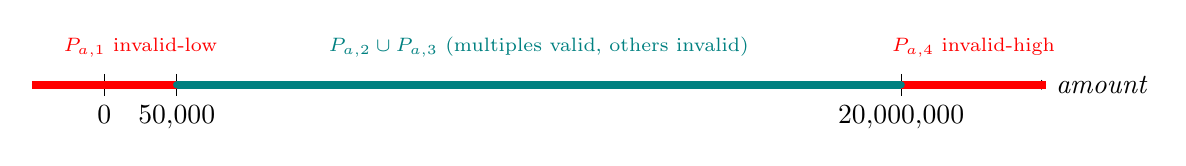
\begin{tikzpicture}[scale=0.92]
\draw[->] (-1,0) -- (13,0) node[right] {\(\mathit{amount}\)};
\draw (0,0.15) -- (0,-0.15) node[below] {$0$};
\draw (1,0.15) -- (1,-0.15) node[below] {$50{,}000$};
\draw (11,0.15) -- (11,-0.15) node[below] {$20{,}000{,}000$};
\draw[line width=3pt, red] (-1,0) -- (0,0);
\draw[line width=3pt, red] (0,0) -- (1,0);
\node[above,red,font=\scriptsize] at (0.5,0.25) {\(P_{a,1}\) invalid-low};
\draw[line width=3pt, teal] (1,0) -- (11,0);
\node[above,teal,font=\scriptsize] at (6,0.25) {\(P_{a,2}\cup P_{a,3}\) (multiples valid, others invalid)};
\draw[line width=3pt, red] (11,0) -- (13,0);
\node[above,red,font=\scriptsize] at (12,0.25) {\(P_{a,4}\) invalid-high};
\foreach \x in {1,2,...,11} \filldraw[teal] (\x,0) circle (1.2pt);
\end{tikzpicture}
\caption{\(\mathit{amount}\) partitioning on a number line (all other inputs
held at their nominal values). Teal tick marks on \([50{,}000,20{,}000{,}000]\)
denote the reachable valid multiples of $50{,}000$; any non-tick integer in
that same visual interval belongs instead to invalid class \(P_{a,3}\).}
\label{fig:atm-amount-line}
\end{figure}

\begin{figure}[H]
\centering
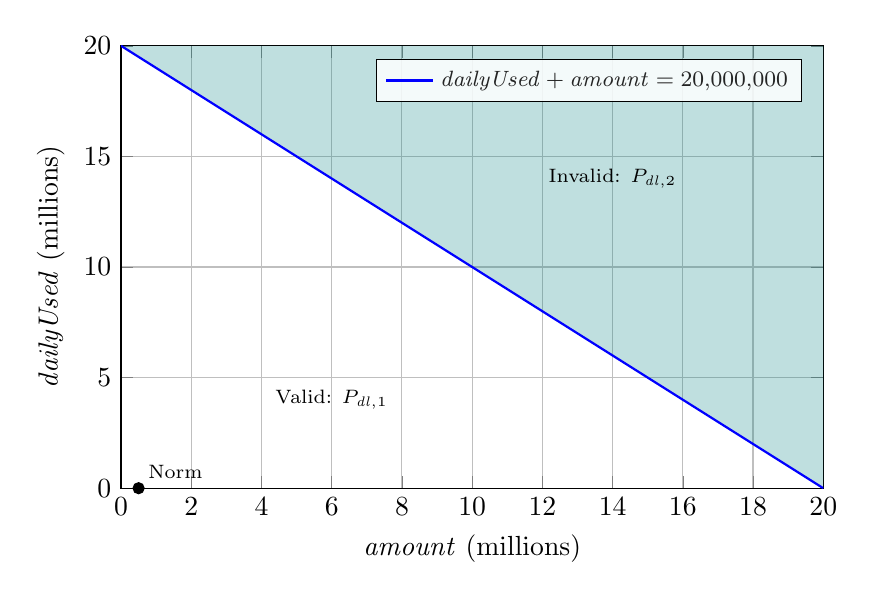
\begin{tikzpicture}
\begin{axis}[
  width=10.5cm, height=7.2cm,
  xlabel={\(\mathit{amount}\) (millions)}, ylabel={\(\mathit{dailyUsed}\) (millions)},
  xmin=0, xmax=20, ymin=0, ymax=20,
  domain=0:20,
  legend pos=north east,
  legend style={font=\footnotesize, fill opacity=0.85},
  grid=both,
]
\addplot[thick, blue] {20-x};
\addlegendentry{\(\mathit{dailyUsed}+\mathit{amount}=20{,}000{,}000\)}
\addplot[name path=upper, draw=none] {20};
\addplot[name path=lim, draw=none] {20-x};
\addplot[teal, opacity=0.25] fill between[of=lim and upper];
\node[font=\scriptsize] at (axis cs:14,14) {Invalid: \(P_{\mathit{dl},2}\)};
\node[font=\scriptsize] at (axis cs:6,4) {Valid: \(P_{\mathit{dl},1}\)};
\addplot[only marks, mark=*, mark size=2pt, black] coordinates {(0.5,0)} node[pos=0,above right,font=\scriptsize]{\(\Norm\)};
\end{axis}
\end{tikzpicture}
\caption{Daily-limit interaction: the derived boundary line
\(\mathit{dailyUsed}+\mathit{amount}=20{,}000{,}000\) in the
\((\mathit{amount},\mathit{dailyUsed})\) plane, with \(\mathit{balance}\),
\(\mathit{accountStatus}\), \(\mathit{isInternal}\) fixed at their nominal
values. This is a 2D projection of the 5-dimensional input space.}
\label{fig:atm-daily-plane}
\end{figure}

\begin{figure}[H]
\centering
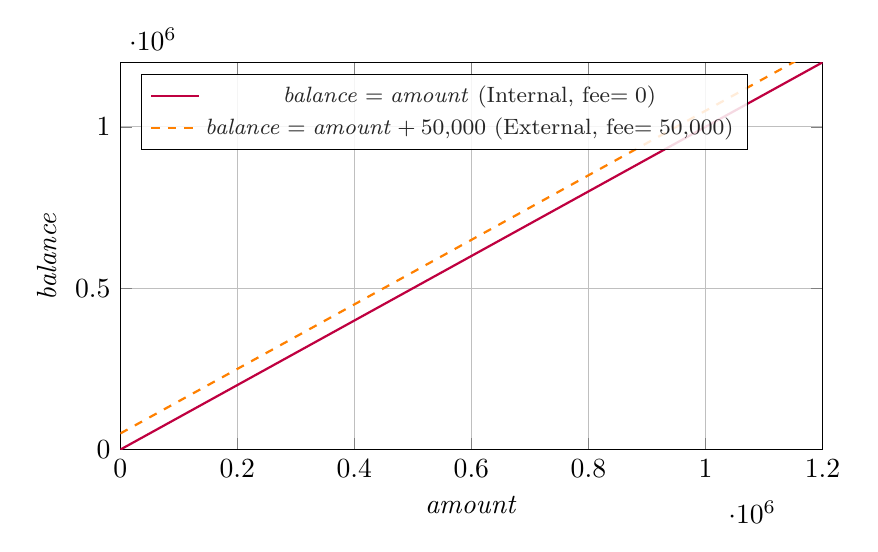
\begin{tikzpicture}
\begin{axis}[
  width=10.5cm, height=6.5cm,
  xlabel={\(\mathit{amount}\)}, ylabel={\(\mathit{balance}\)},
  xmin=0, xmax=1200000, ymin=0, ymax=1200000,
  grid=both,
  legend pos=north west,
  legend style={font=\footnotesize, fill opacity=0.85},
]
\addplot[thick, purple, domain=0:1200000] {x};
\addlegendentry{\(\mathit{balance}=\mathit{amount}\) (Internal, fee\(=0\))}
\addplot[thick, orange, dashed, domain=0:1200000] {x+50000};
\addlegendentry{\(\mathit{balance}=\mathit{amount}+50{,}000\) (External, fee\(=50{,}000\))}
\end{axis}
\end{tikzpicture}
\caption{Balance/fee interaction: the effective balance boundary line shifts
upward by exactly $50{,}000$ when \(\mathit{isInternal}\) flips from
\textsc{True} to \textsc{False}, with \(\mathit{dailyUsed}=0\),
\(\mathit{accountStatus}=\mathrm{Active}\). This is a multi-variable boundary
illustration: the same \((\mathit{amount},\mathit{balance})\) pair can be
Approved or Rejected\_InsufficientBalance purely depending on
\(\mathit{isInternal}\).}
\label{fig:atm-fee-plane}
\end{figure}

\subsection{Boundary Value Analysis}

\paragraph{Amount lower boundary: a discrete range boundary under a
granularity constraint (\(x=50{,}000\)).} R2 is the conjunction of a
\emph{numerical range} condition and a \emph{discrete granularity}
(divisibility) condition, so its boundary cannot be read as a single
continuous inequality edge: $50{,}000$ is not merely ``the smallest number
\(\ge 50{,}000\),'' it is \emph{the first value that is simultaneously
\(\ge 50{,}000\) and a multiple of $50{,}000$}, i.e.\ the first \emph{reachable}
valid amount. Consequently $49{,}999$ fails range \emph{and} would also fail
divisibility if range were somehow relaxed (it is not itself a multiple of
$50{,}000$), so it is classified here by range alone under the fixed
precedence order (range is checked, and fails, before divisibility would
even matter); by contrast $50{,}001$ fails on granularity \emph{alone}
(range holds, divisibility fails) even though it is numerically adjacent to
a valid point. A value that fails range \emph{purely}, with divisibility
never even a candidate distinction, is $0$ (TC-ATM-20, \S4.10), which is
itself a multiple of $50{,}000$ and so isolates the range failure mode
cleanly. These are, taken together, genuinely different kinds of failure
clustered around the same nominal boundary value, not a symmetric \(\pm1\)
perturbation of one inequality:

\begin{table}[H]
\centering
\caption{\(\mathit{amount}\) lower boundary --- discrete range boundary under a granularity constraint}
\begin{tabularx}{\textwidth}{L{2.2cm} L{3.5cm} L{3.3cm} l Y}
\toprule
Range-invalid side & First reachable value & Granularity-invalid side & Nominal & Expected behaviour \\
\midrule
$49{,}999$ (range fails) & $50{,}000$ (valid: range holds \emph{and} divisible) & $50{,}001$ (range holds, granularity fails) & $500{,}000$ & Both invalid sides reject as \texttt{InvalidAmount}; only $50{,}000$ is Approved-eligible \\
\bottomrule
\end{tabularx}
\end{table}

\(\mathit{amount}=0\) is analysed separately (TC-ATM-20, \S4.10) as a
representative deep-invalid value of \(P_{a,1}\) and as the unique test that
isolates a pure range failure (above); it is also the value that
distinguishes mutant M10 (lower bound removed), since $0$ is itself a
multiple of $50{,}000$ and would therefore be wrongly accepted if the lower
bound were dropped.

\paragraph{Amount upper boundary: the same discrete pattern in reverse
(\(x=20{,}000{,}000\)).} By the same reasoning, $20{,}000{,}000$ is the
\emph{last reachable valid amount}: it is simultaneously $\le
20{,}000{,}000$ and a multiple of $50{,}000$. Its two neighbours fail for two
different reasons: $19{,}999{,}999$ fails on granularity alone (it is
in-range but not a multiple of $50{,}000$), while $20{,}000{,}001$ fails on
\emph{both} range and granularity simultaneously (it exceeds the limit
\emph{and} is not a multiple of $50{,}000$), which makes it a poor
representative for isolating the ``too high'' failure mode in particular.
The representative over-range value used below is instead $20{,}050{,}000$
(the next reachable multiple of $50{,}000$ above the limit), which fails on
range grounds alone (divisibility holds) and cleanly isolates that failure
mode from the granularity failure already exercised at $50{,}001$
(TC-ATM-07) and $60{,}000$ (TC-ATM-18, \S4.12); no test in the suite uses
$19{,}999{,}999$ itself, since its role here is illustrative (Table~\ref{tab:atm-amount-hi}), not
a retained test case:

\begin{table}[H]
\centering
\caption{\(\mathit{amount}\) upper boundary --- discrete range boundary under a granularity constraint}
\label{tab:atm-amount-hi}
\begin{tabularx}{\textwidth}{L{3.2cm} L{3.7cm} L{3.2cm} Y}
\toprule
Granularity-invalid side & Last reachable value & Range-invalid side & Expected behaviour \\
\midrule
$19{,}999{,}999$ (in range, not a multiple) &
$20{,}000{,}000$ (valid: range holds \emph{and} divisible) &
$20{,}050{,}000$ (over range, still a multiple) &
Both invalid sides reject as \texttt{InvalidAmount}; TC-ATM-05 places
\(\mathit{balance}=20{,}000{,}000\) so that this boundary value is deterministically Approved \\
\bottomrule
\end{tabularx}
\end{table}

\paragraph{Granularity (divisibility) boundary in the interior of the
range.} Around every reachable multiple \(k\cdot 50{,}000\) strictly inside
\((50{,}000,\,20{,}000{,}000)\), the immediate integer neighbours
\(k\cdot50{,}000 \pm 1\) are non-multiples and hence invalid purely on
granularity grounds, with range never at issue. TC-ATM-07 ($50{,}001$) and
TC-ATM-18 ($60{,}000$, chosen specifically because it is divisible by
$10{,}000$ but not by $50{,}000$, \S4.12/M8) both instantiate this interior
granularity boundary.

\paragraph{Balance boundary (\(\mathit{balance}=\mathit{amount}+\mathit{fee}\)).}
The three points immediately around the threshold $T$ are:
\begin{table}[H]
\centering
\caption{Balance boundary around \(T=\mathit{amount}+\mathit{fee}\)}
\begin{tabularx}{\textwidth}{l l l Y}
\toprule
\(\mathit{balance}=T-1\) & \(\mathit{balance}=T\) & \(\mathit{balance}=T+1\) & Expected \\
\midrule
Rejected\_InsufficientBalance & Approved (boundary satisfies \(\ge\)) & Approved &
R5 is non-strict (\(\ge\)), so equality is the last valid point, not the first invalid one \\
\bottomrule
\end{tabularx}
\end{table}

\paragraph{Daily-limit boundary (\(\mathit{dailyUsed}+\mathit{amount}=20{,}000{,}000\)).}
The three points immediately around this derived sum are:
\begin{table}[H]
\centering
\caption{Daily-limit boundary}
\begin{tabularx}{\textwidth}{l l Y}
\toprule
Sum \(=19{,}999{,}999\) & Sum \(=20{,}000{,}000\) & Sum \(=20{,}000{,}001\) \\
\midrule
Valid (R3 holds) & Valid (R3 holds, equality) & Invalid (Rejected\_DailyLimit) \\
\bottomrule
\end{tabularx}
\end{table}

\paragraph{Status boundary (categorical).} \(\mathrm{Active} \leftrightarrow \mathrm{Frozen}\): since \(D_{status}\) has exactly two members
with no ordering, the ``boundary'' is simply the exhaustive pairwise test of
both values, each otherwise-valid.

\paragraph{Internal/external fee boundary (categorical, but numerically
consequential).} Flipping \(\mathit{isInternal}\) while \(\mathit{amount}\) and
\(\mathit{balance}\) are unchanged can flip the outcome of R5, because it moves
the threshold \(T\) by exactly $50{,}000$ (Figure~\ref{fig:atm-fee-plane}).
This is analysed jointly with the balance boundary in \S4.9, since testing
\(\mathit{isInternal}\) alone (holding \(\mathit{amount}\), \(\mathit{balance}\)
nominal, both far from \(T\)) would never reveal this interaction.

\subsection{Boundary Combinations}

Single-variable BVA is provably insufficient here: a test with
\(\mathit{amount}=50{,}000\) and a separately-chosen ``boundary'' \(\mathit{balance}\)
value taken from \emph{that variable's own} boundary table (e.g.\
\(\mathit{balance}=999{,}999/1{,}000{,}000/1{,}000{,}001\), boundaries of an
unrelated nominal \(T'\)) would never place \(\mathit{balance}\) at the boundary
\emph{that actually matters for this \(\mathit{amount}\)}, namely
\(T=50{,}000+\mathit{fee}\). The combinations below fix that.

\begin{xltabular}{\textwidth}{l L{4.5cm} Y}
\caption{Mandatory ATM boundary combinations} \label{tab:atm-combos}\\
\toprule
Combination & Inputs (others nominal) & Why it matters \\
\midrule
\endfirsthead
\toprule
Combination & Inputs (others nominal) & Why it matters \\
\midrule
\endhead
\bottomrule
\endfoot
C1 & \(\mathit{amount}=50{,}000,\ \mathit{balance}=50{,}000\) &
Amount at its own lower boundary \emph{and} balance at exactly \(T\)
(Internal) simultaneously: both R2 and R5 are boundary-tight at once. \\
\addlinespace
C2 & \(\mathit{amount}=50{,}000,\ \mathit{balance}=50{,}001\) &
Same amount boundary, balance now one unit past \(T\): isolates that R5 alone
flips while R2 stays satisfied. \\
\addlinespace
C3 & \(\mathit{balance}=\mathit{amount}+\mathit{fee}\) \emph{and}
\(\mathit{dailyUsed}+\mathit{amount}=20{,}000{,}000\) simultaneously
(e.g.\ \(\mathit{amount}=500{,}000\), \(\mathit{dailyUsed}=19{,}500{,}000\),
\(\mathit{balance}=500{,}000\), Internal) &
Two independent derived boundaries (R3 and R5) are both exactly tight in the
same test; per the precedence rule, R3 is checked first, so this must still
be Approved only if \emph{both} hold, and any single-bit perturbation of
either boundary must reject for the correspondingly different reason. \\
\addlinespace
C4 & \(\mathit{dailyUsed}+\mathit{amount}=20{,}000{,}001\) \emph{and}
\(\mathit{balance}<\mathit{amount}+\mathit{fee}\) simultaneously (e.g.\
\(\mathit{amount}=500{,}000\), \(\mathit{dailyUsed}=19{,}500{,}001\),
\(\mathit{balance}=499{,}999\), Internal) &
Both R3 \emph{and} R5 fail at once. This is deliberately \emph{not} the
simpler case ``R3 fails, R5 would have passed'': if only R3 failed, checking
R3 before R5 or R5 before R3 would report the same reason either way (R3
fails immediately in the first order; in the second order R5 passes and R3
is then found to fail) -- a single-failure case cannot distinguish the two
orderings at all. Only a \emph{simultaneous} double failure does: checking
R3 first reports Rejected\_DailyLimit, checking R5 first reports
Rejected\_InsufficientBalance. This is therefore the only combination that
actually exercises, and can kill, a precedence-swap mutant (\S4.12, M11). \\
\addlinespace
C5 & $\mathit{amount}=500{,}000,\ \mathit{balance}=500{,}000,\
\mathit{isInternal}=\mathrm{True}$ vs. \(\mathit{isInternal}=\mathrm{False}\)
(balance unchanged) &
Toggling \(\mathit{isInternal}\) alone, at a balance sitting exactly on the
Internal threshold, must flip the outcome from Approved to
Rejected\_InsufficientBalance purely because \(T\) moved from $500{,}000$ to
$550{,}000$ -- direct evidence that isInternal and balance are not
independently testable. \\
\addlinespace
C6 & \(\mathit{isInternal}=\mathrm{False}\), \(\mathit{amount}=500{,}000\),
\(\mathit{balance}=520{,}000\) &
Places \(\mathit{balance}\) strictly between the correct threshold
($550{,}000$) and a plausible wrong-fee threshold ($505{,}000$): the correct
specification rejects (Insufficient), while a mutant using an incorrect fee
constant would approve. Needed because C5's balance ($500{,}000$) sits
below \emph{both} thresholds and cannot distinguish ``fee removed'' from
``fee has the wrong value.'' \\
\addlinespace
C7 & \(\mathit{amount}=0\), others nominal &
The lower range bound and the granularity condition agree that $0$ is
invalid (it is below $50{,}000$), but $0$ is itself a multiple of
$50{,}000$; only a mutant that has actually removed or lowered the range
floor would accept it, making this the unique test able to kill such a
mutant (\S4.12, M10). \\
\addlinespace
C8 & \(\mathit{isInternal}=\mathrm{False}\), \(\mathit{amount}=500{,}000\),
\(\mathit{balance}=580{,}000\) &
Every other External test in the suite (TC-ATM-14, -19) is Rejected, so no
test exercises the External branch's Approved path or distinguishes the
correct fee threshold ($550{,}000$) from a fee that is too \emph{high}
($600{,}000$ if fee were mistakenly $100{,}000$); $580{,}000$ sits strictly
between the two, so the correct specification approves while an
overcharging-fee mutant would reject (\S4.12, M13). \\
\addlinespace
C9 & \(\mathit{accountStatus}=\mathrm{Frozen}\),
\(\mathit{amount}=49{,}999\), others nominal &
R1 \emph{and} R2 fail simultaneously. Exactly as C4 does for R3/R5, this is
the only configuration able to distinguish the specified R1-before-R2
precedence from a reversed one: when only one of R1, R2 fails (as in every
other test), checking either rule first yields the same reported reason, so
only a genuinely simultaneous double failure can kill a precedence-swap
mutant on R1/R2 (\S4.12, M14). \\
\end{xltabular}

\subsection{Test Suite Construction}

Candidate tests were generated from: (i) one representative per equivalence
class in \S4.6 (8 candidates: \(P_{a,1..4}\), \(P_{s,1..2}\) each combined with
otherwise-valid inputs, \(P_{i,1..2}\)); (ii) one test per boundary row in
\S4.8 (roughly 12 candidates); (iii) the nine combinations C1--C9 of \S4.9,
of which C1--C5 were already candidates and C6--C9 were added specifically
because no candidate from (i)/(ii) was able to distinguish mutants M7, M10,
M13, and M14 respectively (\S4.12) -- a concrete instance of mutation
analysis feeding back into test-suite construction. Redundant candidates
(e.g.\ a plain \(P_{a,3}\) representative that coincides with an
already-scheduled divisibility-boundary test) were merged. Five tests were
added, or repurposed from an existing combination, specifically to close a
gap that only the mutation analysis of \S4.12 exposed -- no candidate from
(i)--(iii) could otherwise distinguish the mutant named: TC-ATM-18
(interior granularity at $60{,}000$) for M8, TC-ATM-19 (\(=\)C6) for M7,
TC-ATM-20 (\(=\)C7) for M10, TC-ATM-21 (\(=\)C8) for M13, and TC-ATM-22
(\(=\)C9) for M14. This is a legitimate part of test-suite construction
(mutation analysis feeding back to close a coverage gap), not a change to
the specification. The resulting twenty-two tests are the complete,
non-redundant ATM suite; every value below was computed directly from the
formal specification in \S4.2, not asserted informally. The same
twenty-two tests are listed below; the coverage of every partition and every
boundary by these tests is checked directly after the table.

\begingroup\small\setlength{\tabcolsep}{3pt}\renewcommand{\arraystretch}{1.15}
\begin{xltabular}{\textwidth}{@{}l L{2.3cm} L{2.3cm} L{2.2cm} c Y@{}}
\caption{ATM complete test suite, with full traceability} \label{tab:atm-suite-sample}\\
\toprule
ID & Inputs (\textit{bal / used / amt / status / internal}) & Partition & Boundary & Combo & Expected output / Rationale \\
\midrule
\endfirsthead
\toprule
ID & Inputs (\textit{bal / used / amt / status / internal}) & Partition & Boundary & Combo & Expected output / Rationale \\
\midrule
\endhead
\bottomrule
\endfoot
TC-ATM-01 & 1{,}000{,}000 / 0 / 500{,}000 / Active / True &
\(P_{a,2},P_{\mathit{bal},2},P_{\mathit{dl},1},P_{s,1},P_{i,1}\) & -- & -- &
\textbf{Approved}. Pure nominal baseline; establishes the default valid path. \\
TC-ATM-02 & 1{,}000{,}000 / 0 / 49{,}999 / Active / True & \(P_{a,1}\) &
amount lower boundary, range side (\(-1\)) & -- & \textbf{Rejected\_InvalidAmount}.
One unit below R2's range floor. \\
TC-ATM-03 & 50{,}000 / 0 / 50{,}000 / Active / True & \(P_{a,2}\) &
first reachable amount \(=\) balance \(=T\) & C1 & \textbf{Approved}. Two
boundaries tight simultaneously; if either R2 or R5 were mis-implemented as
strict, this fails. \\
TC-ATM-04 & 50{,}001 / 0 / 50{,}000 / Active / True & \(P_{a,2},P_{\mathit{bal},2}\) &
balance \(=T+1\) & C2 & \textbf{Approved}. Confirms R5 tolerant one unit past \(T\). \\
TC-ATM-05 & 20{,}000{,}000 / 0 / 20{,}000{,}000 / Active / True & \(P_{a,2}\)
(upper edge) & last reachable amount, balance \(=T\) & -- & \textbf{Approved}.
Balance is set exactly to \(T\) so the test is deterministically Approved,
rather than merely ``eligible''; also lands exactly on the daily-limit
boundary (\S4.12, kills M2 and M3). \\
TC-ATM-06 & 1{,}000{,}000 / 0 / 20{,}050{,}000 / Active / True & \(P_{a,4}\) &
upper boundary, range side (\(+50{,}000\)) & -- & \textbf{Rejected\_InvalidAmount}.
Over-range but still a multiple, isolating the range failure from the
granularity failure at TC-ATM-07. \\
TC-ATM-07 & 1{,}000{,}000 / 0 / 50{,}001 / Active / True & \(P_{a,3}\) &
interior granularity boundary & -- & \textbf{Rejected\_InvalidAmount}.
In-range but not a multiple of $50{,}000$. \\
TC-ATM-08 & 499{,}999 / 0 / 500{,}000 / Active / True &
\(P_{\mathit{bal},1}\) & balance \(=T-1\) & -- & \textbf{Rejected\_InsufficientBalance}. \\
TC-ATM-09 & 500{,}000 / 0 / 500{,}000 / Active / True &
\(P_{\mathit{bal},2}\) & balance \(=T\) & -- & \textbf{Approved}. Equality is the
boundary, and it is on the valid side. \\
TC-ATM-10 & 1{,}000{,}000 / 19{,}499{,}999 / 500{,}000 / Active / True &
\(P_{\mathit{dl},1}\) & daily sum \(=20{,}000{,}000-1\) & -- & \textbf{Approved}. \\
TC-ATM-11 & 1{,}000{,}000 / 19{,}500{,}000 / 500{,}000 / Active / True &
\(P_{\mathit{dl},1}\) & daily sum \(=20{,}000{,}000\) & -- & \textbf{Approved}
(equality is valid). \\
TC-ATM-12 & 1{,}000{,}000 / 19{,}500{,}001 / 500{,}000 / Active / True &
\(P_{\mathit{dl},2}\) & daily sum \(=20{,}000{,}000+1\) & -- & \textbf{Rejected\_DailyLimit}. \\
TC-ATM-13 & 1{,}000{,}000 / 0 / 500{,}000 / Frozen / True & \(P_{s,2}\) &
categorical status & -- & \textbf{Rejected\_InvalidAccount}, regardless of
otherwise-perfect inputs (precedence R1 first). \\
TC-ATM-14 & 500{,}000 / 0 / 500{,}000 / Active / False &
\(P_{i,2}\) & fee threshold shift & C5 & \textbf{Rejected\_InsufficientBalance}
-- identical balance/amount to TC-ATM-09, but fee now $50{,}000$ moves \(T\)
to \(550{,}000>\mathit{balance}\). \\
TC-ATM-15 & 500{,}000 / 19{,}500{,}000 / 500{,}000 / Active / True & --
(R3,R5 both tight) & double derived boundary (balance \(=T\) \emph{and} daily
sum \(=20{,}000{,}000\)) & C3 & \textbf{Approved} -- both boundaries satisfied
simultaneously. \\
TC-ATM-16 & 499{,}999 / 19{,}500{,}001 / 500{,}000 / Active / True & --
(R3,R5 both fail) & daily sum \(=20{,}000{,}001\) \emph{and} balance \(<T\)
simultaneously & C4 & \textbf{Rejected\_DailyLimit} -- both R3 and R5 fail;
under the specified precedence (R3 before R5) the reported reason is
DailyLimit. This is the only test able to distinguish the specified
precedence from a reversed one (\S4.12, M11). \\
TC-ATM-17 & \(-100\) / 0 / 500{,}000 / Active / True & invalid
\(\mathit{balance}<0\) (deep invalid, sanity) & -- & -- &
\textbf{Rejected\_InsufficientBalance} -- illustrates that the domain
technically allows a negative balance (e.g.\ an already-overdrawn account)
and the rule still resolves to a single, well-defined output. \\
TC-ATM-18 & 1{,}000{,}000 / 0 / 60{,}000 / Active / True & \(P_{a,3}\) &
interior granularity boundary, chosen to be divisible by \(10{,}000\) but not
\(50{,}000\) & -- & \textbf{Rejected\_InvalidAmount}. Needed because
TC-ATM-07's \(50{,}001\) fails divisibility under \emph{any} plausible modulus
mutant and therefore cannot distinguish the correct modulus from a wrong one
(\S4.12, M8). \\
TC-ATM-19 & 520{,}000 / 0 / 500{,}000 / Active / False & \(P_{\mathit{bal},1}\)
& balance strictly between the correct and an incorrect fee threshold & C6 &
\textbf{Rejected\_InsufficientBalance}. Needed because TC-ATM-14's balance
(\(500{,}000\)) sits below every plausible fee threshold and so cannot
distinguish ``fee removed'' from ``fee has the wrong magnitude''
(\S4.12, M6 vs.\ M7). \\
TC-ATM-20 & 1{,}000{,}000 / 0 / 0 / Active / True & \(P_{a,1}\) & amount \(=0\)
(mandated deep-invalid boundary; also a multiple of \(50{,}000\)) & C7 &
\textbf{Rejected\_InvalidAmount}. The only test able to distinguish a
correctly-enforced lower bound from one that has been removed or lowered to
\(0\) (\S4.12, M10). \\
TC-ATM-21 & 580{,}000 / 0 / 500{,}000 / Active / False &
\(P_{a,2},P_{\mathit{bal},2},P_{i,2}\) & fee threshold, External-Approved &
C8 & \textbf{Approved}. The suite's only Approved External test; balance
sits strictly between the correct threshold ($550{,}000$) and an
overcharging-fee threshold ($600{,}000$), so it is the unique test able to
kill a mutant that charges too \emph{high} a fee (\S4.12, M13). \\
TC-ATM-22 & 1{,}000{,}000 / 0 / 49{,}999 / Frozen / True & \(P_{a,1},P_{s,2}\)
& R1 \emph{and} R2 simultaneously invalid & C9 &
\textbf{Rejected\_InvalidAccount}. R1 and R2 both fail at once; under the
specified precedence (R1 before R2) the reported reason is InvalidAccount.
This is the only test able to distinguish the specified R1-before-R2
precedence from a reversed one (\S4.12, M14). \\
\end{xltabular}
\endgroup

\paragraph{Coverage check.} Tables~\ref{tab:atm-partition-coverage}
and~\ref{tab:atm-boundary-coverage} read the suite in the opposite direction:
starting from each partition (\S4.6) and each boundary (\S4.8--4.9), they name
the tests that exercise it, so that a class or boundary without a test would
be visible as an empty cell.

{\small
\begin{longtable}{L{2.2cm} L{7.2cm} L{1.7cm} L{2.7cm}}
\caption{ATM partition coverage: every class of \S4.6 and a test that represents it} \label{tab:atm-partition-coverage}\\
\toprule
Partition ID & Mathematical definition & Valid / Invalid & Representative test \\
\midrule
\endfirsthead
\toprule
Partition ID & Mathematical definition & Valid / Invalid & Representative test \\
\midrule
\endhead
\bottomrule
\endfoot
$P_{a,1}$ & $\{x\in\mathbb{Z}\mid x<50{,}000\}$ & Invalid & TC-ATM-02 \\
$P_{a,2}$ & $\{x\in\mathbb{Z}\mid 50{,}000\le x\le20{,}000{,}000\wedge x\equiv0\!\!\pmod{50{,}000}\}$ & Valid & TC-ATM-01 \\
$P_{a,3}$ & $\{x\in\mathbb{Z}\mid 50{,}000\le x\le20{,}000{,}000\wedge x\not\equiv0\!\!\pmod{50{,}000}\}$ & Invalid & TC-ATM-07 \\
$P_{a,4}$ & $\{x\in\mathbb{Z}\mid x>20{,}000{,}000\}$ & Invalid & TC-ATM-06 \\
\(P_{\mathit{bal},1}\) & \(\{x\in\mathbb{Z}\mid x<\mathit{amount}+\mathit{fee}\}\) & Invalid & TC-ATM-08 \\
\(P_{\mathit{bal},2}\) & \(\{x\in\mathbb{Z}\mid x\ge\mathit{amount}+\mathit{fee}\}\) & Valid & TC-ATM-09 \\
\(P_{\mathit{dl},1}\) & \(\{(d,a)\mid d+a\le20{,}000{,}000\}\) & Valid & TC-ATM-11 \\
\(P_{\mathit{dl},2}\) & \(\{(d,a)\mid d+a>20{,}000{,}000\}\) & Invalid & TC-ATM-12 \\
\(P_{s,1}\) & \(\{\mathrm{Active}\}\) & Valid & TC-ATM-01 \\
\(P_{s,2}\) & \(\{\mathrm{Frozen}\}\) & Invalid & TC-ATM-13 \\
\(P_{i,1}\) & \(\{\mathrm{True}\}\) (fee\(=0\)) & Valid (numerically neutral) & TC-ATM-01 \\
\(P_{i,2}\) & \(\{\mathrm{False}\}\) (fee\(=50{,}000\)) & Valid (numerically neutral) & TC-ATM-14 \\
\end{longtable}
}
Every listed partition has at least one representative test in the suite
(Table~\ref{tab:atm-suite-sample}); completeness holds because every input value falls in exactly
one listed class per input dimension, and the joint suite covers the
Cartesian combinations identified in \S4.9.

\begin{longtable}{L{1.8cm} L{4.2cm} L{1.6cm} L{2.2cm} L{3.6cm}}
\caption{ATM boundary coverage: every boundary of \S4.8--4.9 and the tests that exercise it} \label{tab:atm-boundary-coverage}\\
\toprule
Boundary ID & Definition & Type & Covered by & Expected change \\
\midrule
\endfirsthead
\toprule
Boundary ID & Definition & Type & Covered by & Expected change \\
\midrule
\endhead
\bottomrule
\endfoot
B-amt-lo & \(\mathit{amount}=50{,}000\) & Input-domain & TC-ATM-02, -03 &
Invalid\(\to\)valid-range \\
B-amt-hi & \(\mathit{amount}=20{,}000{,}000\) & Input-domain & TC-ATM-05, -06 &
Valid-range\(\to\)invalid \\
B-amt-div & \(\mathit{amount}\bmod 50{,}000=0\) & Invalid/\allowbreak valid & TC-ATM-07 &
Multiple\(\to\)non-multiple \\
B-bal & \(\mathit{balance}=\mathit{amount}+\mathit{fee}\) & Derived & TC-ATM-08,
-09, C1/C2 & Rejected\(\to\)Approved \\
B-daily & \(\mathit{dailyUsed}+\mathit{amount}=20{,}000{,}000\) & Derived &
TC-ATM-10, -11, -12 & Approved \(\to\) Rejected\_\allowbreak DailyLimit \\
B-status & \(\mathrm{Active}\leftrightarrow\mathrm{Frozen}\) & Logical &
TC-ATM-13 & Any \(\to\) Rejected\_\allowbreak InvalidAccount \\
B-fee & \(\mathit{isInternal}\) True\(\leftrightarrow\)False & Multi-variable
interaction & TC-ATM-14, C5 & Approved \(\leftrightarrow\) Rejected\_\allowbreak InsufficientBalance \\
B-multi1 & B-bal \(\wedge\) B-daily simultaneously & Multi-variable
interaction & TC-ATM-15/16, C3/C4 & Confirms precedence order (R3/R5) \\
B-fee-hi & \(\mathit{balance}=\mathit{amount}+100{,}000\) (overcharge
threshold) & Multi-variable interaction & TC-ATM-21, C8 & Isolates the
External-Approved path; distinguishes correct fee from an overcharging one \\
B-multi2 & R1 \(\wedge\) R2 simultaneously invalid & Multi-variable
interaction & TC-ATM-22, C9 & Confirms precedence order (R1/R2) \\
B-out & 5-way \(D_{out}\) partition & Output & entire suite & Every rejection
reason is individually reachable \\
\end{longtable}

\subsection{Mutation Model}

\begingroup\small
\begin{xltabular}{\textwidth}{@{}l L{3.5cm} L{3.7cm} L{2.0cm} Y@{}}
\caption{ATM mutants} \label{tab:atm-mutants}\\
\toprule
ID & Original & Mutated & Fault type & Targeted partition/boundary \\
\midrule
\endfirsthead
\toprule
ID & Original & Mutated & Fault type & Targeted partition/boundary \\
\midrule
\endhead
\bottomrule
\endfoot
M1 & \(\mathit{balance}\ge \mathit{amount}+\mathit{fee}\) (R5) &
\(\mathit{balance} > \mathit{amount}+\mathit{fee}\) & Relational operator &
Balance equality boundary (\(T\)) \\
M2 & \(\mathit{dailyUsed}+\mathit{amount}\le 20{,}000{,}000\) (R3) &
\(\mathit{dailyUsed}+\mathit{amount} < 20{,}000{,}000\) & Relational operator &
Daily-limit equality boundary \\
M3 & $20{,}000{,}000$ (upper amount bound, R2) & $19{,}999{,}999$ &
Boundary constant \(-1\) & Amount upper boundary \\
M4 & $20{,}000{,}000$ (upper amount bound, R2) & $20{,}000{,}001$ &
Boundary constant \(+1\) & Amount upper boundary --
\textbf{equivalent mutant} (see discussion below) \\
M5 & Gate requires \emph{both} to hold
(\(\mathrm{R1}\wedge\mathrm{R2}\)) & Gate requires only \emph{either}
(\(\mathrm{R1}\vee\mathrm{R2}\)); R3/R5 unchanged
& Logical connective (AND\(\to\)OR) & Interaction of status and amount
validity (only the R1/R2 gate is mutated; R3, R5 are unaffected) \\
M6 & \(\mathit{fee}=50{,}000\) if External & \(\mathit{fee}=0\) always
(fee removed) & Missing computation & Fee/isInternal interaction \\
M7 & \(\mathit{fee}=50{,}000\) if External & \(\mathit{fee}=5{,}000\) if
External & Wrong constant & Fee magnitude \\
M8 & \(\mathit{amount}\equiv 0 \pmod{50{,}000}\) (R2) &
\(\mathit{amount}\equiv 0 \pmod{10{,}000}\) & Wrong divisibility constant &
Amount divisibility boundary \\
M9 & \(\mathit{accountStatus}=\mathrm{Active}\) (R1) &
\(\mathit{accountStatus}=\mathrm{Frozen}\) (condition reversed) &
Reversed categorical condition & Status boundary \\
M10 & $50{,}000$ (lower amount bound, R2) & $0$ & Boundary constant
(lower bound removed) & Amount lower boundary \\
M11 & Precedence order R1, R2, R3, R5 & Precedence order R1, R2, R5, R3 (R3/R5
swapped) & Control-flow reordering & Multi-failure precedence \\
M12 & \(\mathit{dailyUsed}+\mathit{amount}\le 20{,}000{,}000\) (R3) &
\(\mathit{dailyUsed}\le 20{,}000{,}000\) (amount dropped from sum) &
Arithmetic mutation & Daily-limit derived boundary \\
M13 & \(\mathit{fee}=50{,}000\) if External &
\(\mathit{fee}=100{,}000\) if External & Wrong constant & Fee magnitude
(overcharge direction) \\
M14 & Precedence order R1, R2, R3, R5 & Precedence order R2, R1, R3, R5 (R1/R2
swapped) & Control-flow reordering & Multi-failure precedence (status/amount) \\
\end{xltabular}
\endgroup

\subsection{Test--Mutant Analysis}

Table~\ref{tab:atm-matrix} reports \textbf{analytically expected} killing:
for each (test, mutant) pair, whether the mutant's specification-implied
output for that test's input differs from the original specification's
expected output. \texttt{K} means ``this test's input makes the mutant
compute a different result than the original,'' derived by hand; the matrix
was afterwards re-computed by executing the mutants and matched cell for
cell (\S\ref{sec:atm-exec}).

Every cell below was obtained by substituting the test's five input values
into both the original rule set (\S4.2) and the mutated rule set, evaluating
each of R1--R5 explicitly under the fixed precedence order, and comparing
the two resulting elements of \(D_{out}\); \texttt{K} is recorded only when
the two elements differ. A cell is \texttt{--} when an earlier rule already
fails identically in both the original and the mutant (the mutated rule is
never reached, so it cannot possibly influence the output for that test).

\begin{table}[H]
\centering
\caption{ATM Test\(\times\)Mutant matrix (analytically expected; \texttt{K}=kill, \texttt{S}=survive (reached, no observable difference), \texttt{--}=mutated rule not reached)}
\label{tab:atm-matrix}
\small
\setlength{\tabcolsep}{3pt}
\begin{tabular}{lcccccccccccccc}
\toprule
Test & M1 & M2 & M3 & M4 & M5 & M6 & M7 & M8 & M9 & M10 & M11 & M12 & M13 & M14 \\
\midrule
TC-ATM-01 & S & S & S & S & S & S & S & S & K & S & S & S & S & S \\
TC-ATM-02 & -- & -- & S & S & K & -- & -- & S & K & S & -- & -- & -- & S \\
TC-ATM-03 & K & S & S & S & S & S & S & S & K & S & S & S & S & S \\
TC-ATM-04 & S & S & S & S & S & S & S & S & K & S & S & S & S & S \\
TC-ATM-05 & K & K & K & S & S & S & S & S & K & S & S & S & S & S \\
TC-ATM-06 & -- & -- & S & S & K & -- & -- & S & K & S & -- & -- & -- & S \\
TC-ATM-07 & -- & -- & S & S & K & -- & -- & S & K & S & -- & -- & -- & S \\
TC-ATM-08 & S & S & S & S & S & S & S & S & K & S & S & S & S & S \\
TC-ATM-09 & K & S & S & S & S & S & S & S & K & S & S & S & S & S \\
TC-ATM-10 & S & S & S & S & S & S & S & S & K & S & S & S & S & S \\
TC-ATM-11 & S & K & S & S & S & S & S & S & K & S & S & S & S & S \\
TC-ATM-12 & -- & S & S & S & S & -- & -- & S & K & S & S & K & -- & S \\
TC-ATM-13 & -- & -- & -- & -- & K & -- & -- & -- & K & -- & -- & -- & -- & S \\
TC-ATM-14 & S & S & S & S & S & K & S & S & K & S & S & S & S & S \\
TC-ATM-15 & K & K & S & S & S & S & S & S & K & S & S & S & S & S \\
TC-ATM-16 & -- & S & S & S & S & -- & -- & S & K & S & K & K & -- & S \\
TC-ATM-17 & S & S & S & S & S & S & S & S & K & S & S & S & S & S \\
TC-ATM-18 & -- & -- & S & S & K & -- & -- & K & K & S & -- & -- & -- & S \\
TC-ATM-19 & S & S & S & S & S & K & K & S & K & S & S & S & S & S \\
TC-ATM-20 & -- & -- & S & S & K & -- & -- & S & K & K & -- & -- & -- & S \\
TC-ATM-21 & S & S & S & S & S & S & S & S & K & S & S & S & K & S \\
TC-ATM-22 & -- & -- & -- & -- & S & -- & -- & -- & K & -- & -- & -- & -- & K \\
\bottomrule
\end{tabular}
\end{table}

\textbf{Discussion of key entries.} M1 (R5 strict) is killed exactly by the
four tests that sit precisely on \(\mathit{balance}=T\) (TC-ATM-03, -05, -09,
-15); every other test that reaches R5 has \(\mathit{balance}\ne T\) and so
cannot distinguish \(\ge\) from \(>\), confirming that only an equality-exact
test can kill a strict-relational mutant. M2 is killed exactly by the three
tests with \(\mathit{dailyUsed}+\mathit{amount}=20{,}000{,}000\) precisely
(TC-ATM-05, -11, -15); TC-ATM-16, whose sum is $20{,}000{,}001$ and therefore
already off the boundary on both sides, does \emph{not} kill M2 -- both the
original ($\le$) and the mutant ($<$) rules reject it identically, since
neither reads the sum as exactly $20{,}000{,}000$. M3 is killed only by
TC-ATM-05 (the unique test with \(\mathit{amount}=20{,}000{,}000\) exactly);
\textbf{M4 is an equivalent mutant} (\S4.12 discussion below) and is killed
by no test, correctly. M5 (the R1/R2 gate weakened from AND to OR) is killed
whenever exactly one of R1, R2 is false while the other is true --
TC-ATM-02, -06, -07, -18, -20 (amount invalid, status valid) and TC-ATM-13
(status invalid, amount valid); TC-ATM-13 is the most illustrative case,
since under M5 the OR-gate lets a \emph{frozen} account's withdrawal proceed
to, and pass, R3/R5, so the mutant wrongly \emph{approves} it, which is a
qualitatively worse failure than the amount-invalid cases (a categorical
precondition is silently bypassed, not merely an off-by-one on a numeric
range) -- and it is precisely because TC-ATM-13 tests the \emph{complete}
four-rule predicate on a Frozen account, rather than status in isolation,
that it is able to expose this. M9 (reversed status condition) is killed by
\emph{every} test in the suite: on the nineteen Active-status tests the
mutant instantly emits
Rejected\_InvalidAccount, which differs from each test's actual (non-
InvalidAccount) expected output, while on the one Frozen test (TC-ATM-13)
the mutant does the mirror-image wrong thing and approves it. This
universal kill rate is an expected property of a coarse, single-bit
categorical reversal on a field the suite deliberately keeps at its valid
value almost everywhere, not evidence of a flawed matrix. M6 and M7 both
mutate only the \(\mathit{isInternal}=\mathrm{False}\) branch of R4, so on
every Internal test that reaches R4/R5, the fee rule is still executed but
computes the identical value ($\mathit{fee}=0$) under both the original and
either mutant, and both columns are correctly \texttt{S} (reached, no
observable difference) there -- not \texttt{--}, since R4 is not skipped,
only its unmutated branch is taken. TC-ATM-14 (\(\mathit{balance}=500{,}000\),
External) kills M6 (fee removed) but \emph{survives} M7 (fee reduced to
$5{,}000$), because $500{,}000$ is below \emph{both} the correct threshold
($550{,}000$) and the wrong one ($505{,}000$); only TC-ATM-19
(\(\mathit{balance}=520{,}000\), strictly between the two thresholds) kills
M7. M8 (wrong divisibility modulus) is killed only by TC-ATM-18
(\(\mathit{amount}=60{,}000\), divisible by $10{,}000$ but not $50{,}000$);
TC-ATM-07 (\(\mathit{amount}=50{,}001\)) is divisible by neither modulus and
is therefore rejected identically by the original and the mutant -- a
concrete instance of why a mutant-killing claim must be verified by
substitution rather than assumed from the mutant's superficial description.
M10 (lower bound removed) is killed only by TC-ATM-20
(\(\mathit{amount}=0\)): every other amount below $50{,}000$ present in the
suite (TC-ATM-02, $49{,}999$) is also non-divisible by $50{,}000$ and so
remains invalid even under the weakened lower bound, whereas $0$ is itself a
multiple of $50{,}000$ and is therefore uniquely capable of exposing a
missing or lowered floor. M11 (precedence swap) is killed only by
TC-ATM-16, the sole test in which R3 \emph{and} R5 fail simultaneously;
TC-ATM-12 (R3 alone fails) and TC-ATM-08/-17 (R5 alone fails) all survive
M11, because when only one of the two rules fails, checking it first or
second yields the same reported reason either way (\S4.9's discussion of
C4 proves this algebraically for all four pass/fail combinations). M12
(amount dropped from the daily-limit sum) is killed by TC-ATM-12 and
TC-ATM-16, both of which have \(\mathit{dailyUsed}\) alone below
$20{,}000{,}000$ while \(\mathit{dailyUsed}+\mathit{amount}\) exceeds it --
the exact condition under which ignoring \(\mathit{amount}\) in the sum
changes R3 from failing to (incorrectly) passing. M13 (fee overcharged to
$100{,}000$) is killed only by TC-ATM-21, the sole test with
\(\mathit{balance}\) strictly between the correct External threshold
($550{,}000$) and the overcharging threshold ($600{,}000$); TC-ATM-14 and
TC-ATM-19, the suite's other two External tests, both have
\(\mathit{balance}\) below \emph{both} thresholds and so are rejected
identically under the original rule and M13, exactly mirroring why TC-ATM-14
alone could not distinguish M6 from M7. M14 (R1/R2 precedence swap) is
killed only by TC-ATM-22, the sole test in which R1 \emph{and} R2 fail
simultaneously; every other test has at most one of R1, R2 false, and (by
the same algebraic argument \S4.9 gives for C4/M11) checking either rule
first then yields the same reported reason, so M14 -- structurally the
same class of mutant as M11, but on the other adjacent rule pair -- can only
be exposed by a genuine double failure of that specific pair.

Of the fourteen mutants, M4 is the one \textbf{equivalent mutant}: because
every valid amount is already a multiple of $50{,}000$, and $50{,}000$ does
not divide $20{,}000{,}001$, raising the upper bound from $20{,}000{,}000$
to $20{,}000{,}001$ admits no additional value into the valid amount set
under any test, so the mutant computes the identical output as the original
specification for every possible input, not merely for the tests in this
suite. It is excluded from the non-equivalent-mutant denominator of the
mutation-score definition in \S2.5. All thirteen remaining mutants
(M1--M3, M5--M14) are killed by at least one test in the twenty-two-test
suite, so, restricted to those thirteen non-equivalent mutants, this
analytically expected matrix supports full (\(13/13\)) expected coverage;
this is a claim about the \emph{design} of the suite against the stated
specification (its executed confirmation and a tool-measured score on an
independent mutant population are reported in
\S\ref{sec:atm-exec}), and (per Section~\ref{sec:limitations}) the
mutant set was itself constructed with knowledge of the suite's boundaries,
so this full coverage should not be read as unbiased evidence that boundary
tests generally dominate interior ones.

\subsection{Executed Validation}
\label{sec:atm-exec}

This subsection reports the executed stage of \S\ref{sec:exec-method} for the
ATM validator.

\paragraph{Implementation decisions.} The specification leaves two points
open, so the implementation makes an explicit choice for each and tests it.
First, \(\mathit{dailyUsed}<0\), which \S4.2 excludes from the domain, raises
an argument-range error instead of returning an element of \(D_{out}\); this
check runs before R1, so a frozen account with a negative
\(\mathit{dailyUsed}\) also raises it. Second, R3 is evaluated in the
rearranged form \(\mathit{dailyUsed}>20{,}000{,}000-\mathit{amount}\). It is
equivalent to R3 for every input that reaches it (R2 has already bounded
\(\mathit{amount}\)), but unlike the direct sum it cannot overflow when
\(\mathit{dailyUsed}\) is close to the largest representable integer; the
specification does not address overflow.

\paragraph{Suite execution.} All 87 ATM tests passed (0.48~s): the 22
designed tests TC-ATM-01--22, 18 supplementary boundary and guard tests,
39 matrix-reproduction checks and 8 properties
(Table~\ref{tab:emp-layers}).

\paragraph{Matrix reproduction.} All 14 columns of
Table~\ref{tab:atm-matrix} were reproduced exactly: every \texttt{K} cell is
reproduced, and no test kills a mutant that the matrix marks \texttt{S} or
\texttt{--}. The executed score is therefore \(13/13\) non-equivalent
mutants, as derived in \S4.12. The equivalence of M4 was additionally checked
by executing the original and M4 for every integer amount in
\([-100{,}000,\ 20{,}200{,}000]\) (20{,}300{,}001 values, all other rules
passing); no output differed. The reproduction depends on one reading of
mutant semantics that Table~\ref{tab:atm-mutants} states only informally: for
M5 (\(\mathrm{R1}\wedge\mathrm{R2}\to\mathrm{R1}\vee\mathrm{R2}\)), a single
failure of R1 or R2 lets evaluation continue to R3 and R5, while a double
failure is reported as Rejected\_InvalidAccount (R1 first). This is the
reading under which TC-ATM-22 survives M5, as Table~\ref{tab:atm-matrix}
states.

\paragraph{Tool-generated mutants.} Stryker.NET generated 23 mutants; one was
ignored by the tool as a redundant block removal, and all other 22 were
killed (0 survived; measured mutation score 100\,\%). By operator, the killed
mutants are equality 10, conditional 4, arithmetic 3, logical 2, negation 2
and statement removal 1. The designed suite alone kills 21 of the 22. The
one it does not kill removes the \(\mathit{dailyUsed}\ge0\) guard; that input
lies outside the domain of \S4.2, so by construction no designed test can
reach it, and it is killed by the supplementary guard tests. Every
tool-generated mutant inside the modelled domain, including the relational
mutants on \(\mathit{balance}<T\) and on the rearranged R3, is killed by the
designed suite.

\subsection{Case Study Discussion}

The ATM case study demonstrates that even a specification built from five
apparently independent business rules produces a joint valid region that is
the \emph{intersection}, not the union, of five per-variable conditions --
and that two of the five rules (R3, R5) are defined over sums/derived
thresholds rather than raw inputs. The single most important lesson is
Figure~\ref{fig:atm-fee-plane}: a categorical, seemingly unrelated input
(\(\mathit{isInternal}\)) silently relocates a numeric boundary
(\(\mathit{balance}\ge T\)) by a fixed offset, so no amount of independently
maximal single-variable coverage of \(\mathit{isInternal}\) and \(\mathit{balance}\)
would ever exercise the case where that relocation is exactly what determines
the outcome.

%=================================================================
\section{Case Study II: Quadratic Equation Solver}
%=================================================================

\subsection{Problem Context}
Given integer coefficients \(a,b,c\), classify the number and nature of the
real solutions of \(ax^2+bx+c=0\). Unlike the ATM case, the three inputs here
are not coupled by separate policy rules but by a single algebraic identity
-- the discriminant -- whose sign alone determines the qualitative output
once the leading-coefficient degeneracy (\(a=0\)) has been handled.

\subsection{Formal Specification}
\[
\mathit{Solve}(a,b,c) \to D_{out}, \qquad a,b,c\in\mathbb{Z}.
\]
\textbf{Bounded domain (assumption, adopted to make systematic testing
tractable).}
\[
D_a=D_b=D_c=\{x\in\mathbb{Z}\mid -100\le x\le 100\}, \qquad D = D_a\times D_b\times D_c.
\]
This bound is adopted purely to make BVA over \(a,b,c\)'s own domain edges
well-defined (Section~5.8); the classification logic itself (below) does not
depend on this bound and would apply unchanged for any \(a,b,c\in\mathbb{Z}\).

\textbf{Case A --- \(a\ne 0\) (quadratic).} Define \(\Delta = b^2-4ac\).
\begin{align}
\Delta<0 &\Rightarrow \mathrm{NoRealRoots}\\
\Delta=0 &\Rightarrow \mathrm{OneRepeatedRealRoot}\\
\Delta>0 &\Rightarrow \mathrm{TwoDistinctRealRoots}
\end{align}

\textbf{Case B --- \(a=0\) (degenerates to linear \(bx+c=0\)).}
\begin{align}
b\ne 0 &\Rightarrow \mathrm{OneLinearRoot}\\
b=0,\ c\ne 0 &\Rightarrow \mathrm{NoSolution}\\
b=0,\ c=0 &\Rightarrow \mathrm{InfinitelyManySolutions}
\end{align}

\textbf{Output domain.}
\begin{multline*}
D_{out}=\{\mathrm{NoRealRoots},\ \mathrm{OneRepeatedRealRoot},\
\mathrm{TwoDistinctRealRoots},\\
\mathrm{OneLinearRoot},\ \mathrm{NoSolution},\
\mathrm{InfinitelyManySolutions}\}
\end{multline*}
\textbf{Assumption.} The specification asks only for the real-root
\emph{classification}, not the numeric roots themselves, and does not ask the
solver to distinguish complex-conjugate roots by value; ``no real roots''
covers the entire \(\Delta<0\) region without further subdivision, since the
problem statement gives no requirement to report complex root values.

\subsection{Input and Output Domains}

\begin{table}[H]
\centering
\caption{Quadratic solver domains}
\begin{tabularx}{\textwidth}{l l Y}
\toprule
Input & Domain & Note \\
\midrule
\(a\) & \(\{-100,\dots,100\}\subset\mathbb{Z}\) & Leading coefficient; \(a=0\) is the case-split boundary \\
\(b\) & \(\{-100,\dots,100\}\subset\mathbb{Z}\) & Linear coefficient \\
\(c\) & \(\{-100,\dots,100\}\subset\mathbb{Z}\) & Constant term \\
\bottomrule
\end{tabularx}
\end{table}

The output domain's six labels are mutually exclusive and, together with
Cases A/B above, collectively exhaustive over all of \(D\): every
\((a,b,c)\in D\) falls into exactly one of \(a\ne0\wedge\Delta\lessgtr0/=0\) or
\(a=0\wedge(b\ne0\ \text{or}\ (b=0\wedge c\lessgtr0/=0))\).

\subsection{Constraints and Dependencies}

\(a\), \(b\), \(c\) are not independently meaningful to the output: the output is a
function of the single derived quantity \(\Delta=b^2-4ac\) when \(a\ne0\), and of
a nested categorical case split on \(b,c\) when \(a=0\). Formally,
\[
\mathit{Solve}(a,b,c) = g\big(\mathbf{1}[a=0],\ b,\ c,\ \Delta(a,b,c)\big)
\]
i.e.\ the output factors through \(\Delta\) (and the \(a=0\)/\(b=0\)/\(c=0\)
indicators), not through \(a,b,c\) individually -- exactly analogous to the ATM
case's factoring through \(\mathit{fee}\) and \(\mathit{dailyUsed}+\mathit{amount}\).

\subsection{Representative and Nominal Configurations}

A single nominal tuple cannot represent both the quadratic and linear
behavioural regions (they are disjoint on \(a=0\) vs.\ \(a\ne0\)), nor the three
qualitatively different quadratic outcomes. It is also necessary, following
\S2.3, to keep two conceptually different kinds of representative value
apart: a \emph{nominal/interior} configuration sits safely inside a
partition, away from every boundary of that partition, whereas a
\emph{canonical boundary} configuration is deliberately placed on, or
immediately adjacent to, a behavioural boundary. \(\Delta=0\) and \((0,0,0)\) are
boundary configurations, not nominal ones, and are labelled as such below
rather than folded into a single undifferentiated ``baseline'' table.

\begin{table}[H]
\centering
\caption{Nominal (interior) configurations}
\label{tab:quad-norms}
\begin{tabularx}{\textwidth}{l c c c Y}
\toprule
Configuration & \(a\) & \(b\) & \(c\) & Justification (why it is deep interior for its region) \\
\midrule
Two-root nominal & $1$ & $7$ & $6$ & \(\Delta=49-24=25>0\), far from \(\Delta=0\); factors as \((x+1)(x+6)\) -- unremarkable two-root case \\
No-real-roots nominal & $1$ & $1$ & $10$ & \(\Delta=1-40=-39<0\), far from \(\Delta=0\) -- unremarkable no-real-roots case \\
Linear nominal & $0$ & $2$ & \(-4\) & \(a=0\) is fixed here only because it is the case-defining value for this branch (Case B); \(b=2\ne0\) is chosen deep away from the nested \(b=0\)/\(c=0\) boundaries inside that branch \\
\bottomrule
\end{tabularx}
\end{table}

\begin{table}[H]
\centering
\caption{Canonical boundary configurations}
\label{tab:quad-boundary-configs}
\begin{tabularx}{\textwidth}{l c c c Y}
\toprule
Configuration & \(a\) & \(b\) & \(c\) & Justification (why it is deliberately on/near a boundary) \\
\midrule
Repeated-root boundary & $1$ & $2$ & $1$ & \(\Delta=4-4=0\) exactly -- the central derived boundary itself, \emph{not} an interior value \\
No-real-roots, boundary-adjacent & $1$ & $1$ & $1$ & \(\Delta=1-4=-3\), the nearest reachable negative discriminant (\S5.8) \\
Two-distinct-roots, boundary-adjacent & $1$ & $3$ & $2$ & \(\Delta=9-8=1\), the nearest reachable positive discriminant (\S5.8) \\
No-solution boundary & $0$ & $0$ & $5$ & \(a=0,b=0,c\ne0\): on the nested \(b=0\) boundary inside Case B \\
Degenerate multi-boundary & $0$ & $0$ & $0$ & \(a=0\wedge b=0\wedge c=0\) simultaneously: three nested boundaries coincide at a single point \\
\bottomrule
\end{tabularx}
\end{table}

Each nominal configuration is ``ordinary'' for its region precisely because
its \(\Delta\) (or, for the linear branch, its \(b,c\)) sits far from every
boundary of that region; each boundary configuration is ordinary in the
opposite sense -- it is chosen \emph{because} it sits on or immediately next
to a boundary, and must therefore never be described as ``deep'' or
``interior.'' TC-QE-01 (\S5.10) is built from the two-root nominal
configuration; TC-QE-02, -03, -07, -05, -06 are built from the boundary
configurations.

\subsection{Equivalence Partitioning}

\paragraph{\(a\).}
\(P_{a^-}=\{a\in D_a\mid a<0\}\), \(P_{a^0}=\{a\in D_a\mid a=0\}\),
\(P_{a^+}=\{a\in D_a\mid a>0\}\) -- exhaustive, mutually exclusive.

\paragraph{Discriminant partitions (for \(a\ne0\), i.e.\ restricted to
\(P_{a^-}\cup P_{a^+}\)).}
\begin{align}
P_{\Delta^-} &= \{(a,b,c)\in D\mid a\ne0,\ \Delta<0\}\\
P_{\Delta^0} &= \{(a,b,c)\in D\mid a\ne0,\ \Delta=0\}\\
P_{\Delta^+} &= \{(a,b,c)\in D\mid a\ne0,\ \Delta>0\}
\end{align}
These three are exhaustive and mutually exclusive over \(\{a\ne0\}\) because
\(\Delta<0,=0,>0\) exhaust \(\mathbb{Z}\)'s trichotomy.

\paragraph{Nested partitions for \(a=0\) (linear degeneration).}
\begin{align}
P_{b\ne0} &= \{(0,b,c)\in D\mid b\ne0\} &\Rightarrow \mathrm{OneLinearRoot}\\
P_{b0,c\ne0} &= \{(0,0,c)\in D\mid c\ne0\} &\Rightarrow \mathrm{NoSolution}\\
P_{b0,c0} &= \{(0,0,0)\} &\Rightarrow \mathrm{InfinitelyManySolutions}
\end{align}
\(P_{b\ne0}\cup P_{b0,c\ne0}\cup P_{b0,c0} = \{0\}\times D_b\times D_c\)
exactly, with the three classes pairwise disjoint by construction (first
split on \(b\), then on \(c\)) -- this is a genuinely \emph{nested} partition,
not a flat one, and must be represented as such (a flat partition of \(a=0\)
into ``\(b=0\)'' / ``\(b\ne0\)'' would miss the further \(c\)-split that
distinguishes NoSolution from InfinitelyManySolutions).

\paragraph{Joint valid region.} Every \((a,b,c)\in D\) is valid input (there is
no ``invalid'' input class here -- any integer triple is a legitimate query
to the classifier); \(D\) itself is partitioned, not filtered, by
\(P_{a^0}\cup P_{a^-}\cup P_{a^+}\), each further sub-partitioned as above.

\subsection{Partition Diagrams}

\begin{figure}[H]
\centering
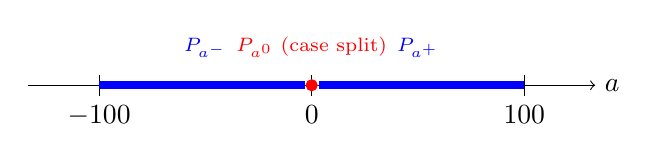
\begin{tikzpicture}[scale=0.9]
\draw[->] (-4,0) -- (4,0) node[right] {\(a\)};
\draw (-3,0.15)--(-3,-0.15) node[below]{\(-100\)};
\draw (0,0.15)--(0,-0.15) node[below]{$0$};
\draw (3,0.15)--(3,-0.15) node[below]{$100$};
\draw[line width=3pt, blue] (-3,0)--(-0.1,0);
\node[above,blue,font=\scriptsize] at (-1.5,0.25) {\(P_{a^-}\)};
\filldraw[red] (0,0) circle (2.2pt);
\node[above,red,font=\scriptsize] at (0,0.25) {\(P_{a^0}\) (case split)};
\draw[line width=3pt, blue] (0.1,0)--(3,0);
\node[above,blue,font=\scriptsize] at (1.5,0.25) {\(P_{a^+}\)};
\end{tikzpicture}
\caption{One-dimensional partition of \(a\). \(a=0\) is a single, isolated point
that is not merely a boundary between two numeric ranges but the switch
between two entirely different classification algorithms (quadratic vs.\
linear).}
\label{fig:quad-a-line}
\end{figure}

\begin{figure}[H]
\centering
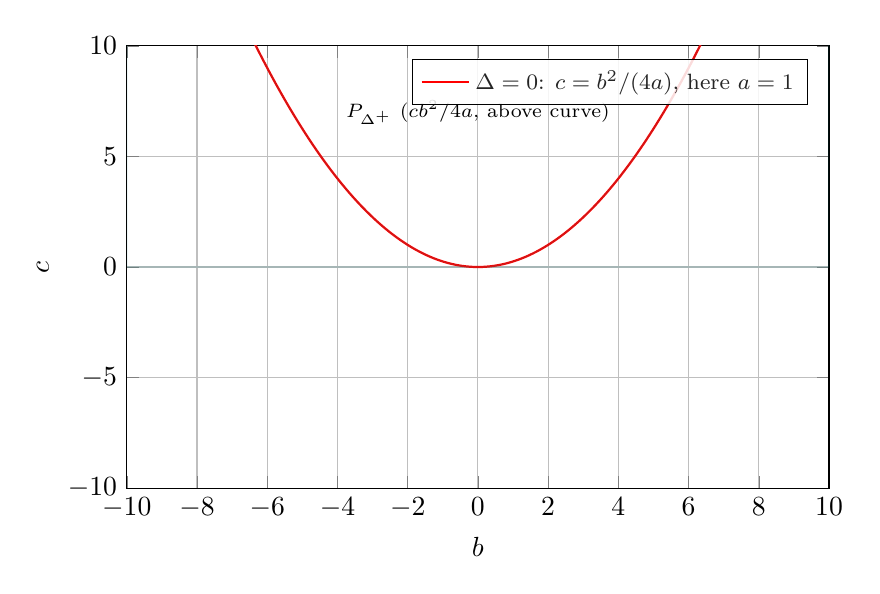
\begin{tikzpicture}
\begin{axis}[
  width=10.5cm, height=7.2cm,
  xlabel={\(b\)}, ylabel={\(c\)},
  xmin=-10, xmax=10, ymin=-10, ymax=10,
  grid=both,
  legend pos=north east,
  legend style={font=\footnotesize, fill opacity=0.85},
  domain=-10:10,
]
\addplot[thick, red, samples=200] {(x^2)/4};
\addlegendentry{\(\Delta=0\): \(c=b^2/(4a)\), here \(a=1\)}
\addplot[teal, opacity=0.2, domain=-10:10, samples=100] {(x^2)/4} \closedcycle;
\node[font=\scriptsize] at (axis cs:0,7) {\(P_{\Delta^+}\) ($cb^2/4a$, above curve)};
\end{axis}
\end{tikzpicture}
\caption{Conceptual \((b,c)\) slice at fixed \(a=1\), showing the discriminant
curve \(b^2-4c=0\) (equivalently \(c=b^2/4\)). This is a 2D \emph{slice} of the
3D \((a,b,c)\) space with \(a\) held fixed at $1$ -- it is not an exact picture
of the full discriminant surface \(b^2-4ac=0\) in 3D, only one cross-section
of it; the curve's shape (and even its convexity direction) changes with the
sign and magnitude of \(a\).}
\label{fig:quad-delta-slice}
\end{figure}

\subsection{Boundary Value Analysis}

\paragraph{Important derived boundary: \(\Delta=0\).}
\emph{This is a joint boundary in \((a,b,c)\)-space, not a boundary of \(b\) or
\(c\) alone.} The surface \(b^2-4ac=0\) is two-dimensional inside the
3-dimensional domain \(D\); ``crossing'' it can be achieved by moving any one
of \(a\), \(b\), or \(c\) while holding the other two fixed, and each such move
constitutes a legitimate boundary test.

\paragraph{Discrete-domain reachability of \(\Delta\) near zero.}
Because \(a,b,c\in\mathbb{Z}\): for any integer \(b\), \(b^2\equiv 0\) or
\(1\pmod4\) (even \(b\): \(b^2\equiv0\); odd \(b\): \(b^2\equiv1\)); and $4ac\equiv
0\pmod4$ always. Therefore
\[
\Delta = b^2-4ac \equiv 0 \text{ or } 1 \pmod 4.
\]
Consequently \(\Delta=-1\) and \(\Delta=-2\) are \textbf{not attainable} for any
integer \(a,b,c\) -- a naive ``test \(\Delta=-1,0,+1\)'' BVA rule would silently
select an impossible input and produce a vacuous, non-executable test case.
The nearest reachable values below and above zero must instead be identified
by construction:

\begin{table}[H]
\centering
\caption{Reachable discriminant values near the boundary, with witnesses}
\label{tab:quad-reach}
\begin{tabularx}{\textwidth}{l c Y}
\toprule
Target \(\Delta\) & Witness \((a,b,c)\) & Check \\
\midrule
\(-3\) (nearest reachable negative) & \((1,1,1)\) & \(1-4=-3\) \\
\(-4\) (also reachable) & \((1,0,1)\) & \(0-4=-4\) \\
$0$ (boundary) & \((1,2,1)\) & \(4-4=0\) \\
$1$ (nearest reachable positive) & \((1,3,2)\) & \(9-8=1\) \\
$4$ (also reachable, \(\equiv0\)) & \((1,4,3)\) & \(16-12=4\) \\
\bottomrule
\end{tabularx}
\end{table}

The witnesses above establish that \(-3\), $0$, and $1$ are all reachable, but
the crossing sequence used in \S5.9 to demonstrate the qualitative
transition (Q7) instead uses \((1,1,1)\to(1,2,1)\to(1,3,1)\), i.e.\ \(a=1\) and
\(c=1\) held fixed and \emph{only} \(b\) incremented (\(1\to2\to3\)): this gives
discriminants \(-3\to0\to5\). Both \(-3\) and $5$ are reachable (\(-3\equiv1\),
\(5\equiv1\pmod4\)), and the sequence is a genuinely single-variable crossing,
unlike a sequence that changes \(c\) partway through, which would conflate a
\(b\)-driven and a \(c\)-driven step and no longer isolate the effect of a
single coefficient.

\paragraph{Coefficient domain boundaries.} The domain extremes and
case-split neighbours \(a,b,c \in \{-100,-1,0,1,100\}\) are the candidate
\emph{direct} boundaries of \(D_a,D_b,D_c\) identified by Stage~3 of the
methodology (\S3.3) -- but these do not all carry equal behavioural weight,
and only the behaviourally significant subset
(Table~\ref{tab:quad-coeff-boundaries} below) is retained in the final suite
(\S5.10); a domain-extreme value with no distinct branch of its own is not
worth a dedicated test. \(a=-100\) or \(a=100\) tests only that the
classifier
accepts the domain's extreme leading coefficients (no distinct branch is
taken there beyond ordinary \(a\ne0\) processing); \(a=0\) and \(a=1\) (its nearest
non-zero neighbour) are far more significant because they straddle the
\emph{behavioural} (case-split) boundary, not merely a domain-range boundary.
\(b=0\) and \(c=0\) are significant only in conjunction with \(a=0\) (they gate the
nested linear/no-solution/infinite-solutions split); when \(a\ne0\), \(b=0\) or
\(c=0\) individually carry no special status beyond their ordinary contribution
to \(\Delta\).

\begin{table}[H]
\centering
\caption{Direct coefficient boundaries vs.\ their behavioural significance}
\label{tab:quad-coeff-boundaries}
\begin{tabularx}{\textwidth}{l L{4.5cm} Y}
\toprule
Value & Domain-edge significance & Behavioural significance \\
\midrule
\(a=-100,100\) & Domain extremes & None beyond ordinary \(a\ne0\) path \\
\(a=-1,1\) & Nearest neighbours of \(a=0\) & High -- adjacent to the case-split \\
\(a=0\) & Interior of \(D_a\) & Maximal -- switches algorithm entirely \\
\(b=0\) (with \(a\ne0\)) & Interior of \(D_b\) & Low -- ordinary \(\Delta\) contribution \\
\(b=0\) (with \(a=0\)) & Interior of \(D_b\) & Maximal -- gates NoSolution vs.\ InfinitelyMany \\
\(c=0\) (with \(a\ne0\)) & Interior of \(D_c\) & Low -- ordinary \(\Delta\) contribution \\
\(c=0\) (with \(a=0,b=0\)) & Interior of \(D_c\) & Maximal -- selects InfinitelyManySolutions \\
\bottomrule
\end{tabularx}
\end{table}

\subsection{Boundary Combinations}

\begin{table}[H]
\centering
\caption{Mandatory quadratic boundary combinations}
\label{tab:quad-combos}
\begin{tabularx}{\textwidth}{l L{4.5cm} Y}
\toprule
Combination & Tuple & Why it matters \\
\midrule
Q1 & \((0,0,0)\) & Deepest degenerate point: all three coefficients zero simultaneously. \\
\addlinespace
Q2 & \((0,0,5)\) & \(a=0,b=0,c\ne0\): isolates NoSolution from InfinitelyManySolutions, which differ only in \(c\). \\
\addlinespace
Q3 & \((0,3,-1)\) & \(a=0,b\ne0\): linear case, \(c\) irrelevant to branch selection once \(b\ne0\). \\
\addlinespace
Q4 & \((1,1,1)\) & \(a\ne0,\Delta<0\) (reachable, \(\Delta=-3\)). \\
\addlinespace
Q5 & \((1,2,1)\) & \(a\ne0,\Delta=0\) (repeated root, boundary). \\
\addlinespace
Q6 & \((1,3,2)\) & \(a\ne0,\Delta>0\) (reachable, \(\Delta=1\)). \\
\addlinespace
Q7 & \((1,1,1)\to(1,2,1)\to(1,3,1)\) & Crossing tuple: holding \(a=1\) and \(c=1\)
fixed and increasing only \(b\) (\(1\to2\to3\)) drives \(\Delta\) through
\(-3\to0\to5\), i.e.\ through
\(\mathrm{NoRealRoots}\to\mathrm{OneRepeatedRealRoot}\to\mathrm{TwoDistinctRealRoots}\)
under a genuinely single-variable (\(b\)-only) change -- the qualitative-change
demonstration required by \S5.8/\S\ref{sec:lessons}. \\
\addlinespace
Q8 & \((2,4,2)\) vs.\ \((1,2,1)\) & Same \(\Delta=0\) boundary reached via a
\emph{different} coefficient combination (both \(a\) and \(c\) doubled): shows
\(\Delta=0\) is a genuinely joint condition, not tied to one specific
\((a,b,c)\) triple. \\
\addlinespace
Q9 & \((-1,0,1)\) & \(a<0\) combined with \(\Delta = 0-4(-1)(1)=4>0\): confirms
sign of \(a\) does not change the discriminant classification logic itself. \\
\bottomrule
\end{tabularx}
\end{table}

Single-variable testing is insufficient here in the strongest possible sense:
holding \(a\) and \(c\) at any fixed nominal value and only varying \(b\) across
its own domain boundary values (\(-100,-1,0,1,100\)) will, for almost all
fixed \((a,c)\), never once land on \(\Delta=0\), because \(\Delta=0\) is a
one-dimensional curve inside a 2D \((b,c)\) slice (for fixed \(a\)), and a
domain-boundary value of \(b\) chosen without reference to \(a,c\) has no
reason to be one of the (at most two) roots of \(b^2=4ac\). Only a boundary-combination
test that solves for one variable in terms of the other two (as Q5, Q7, Q8
do) can reliably hit the derived boundary.

\subsection{Test Suite Construction}

Candidates were generated from: (i) the \(a\)-partition (3 classes) and nested
\(a=0\) partitions (3 sub-classes); (ii) the \(\Delta\)-partition (3 classes);
(iii) the domain-edge boundaries of \(a,b,c\)
(Table~\ref{tab:quad-coeff-boundaries}, \S5.8, filtered to those with real
behavioural significance -- not every coefficient boundary is equally
meaningful); (iv) the nine
combinations Q1--Q9; (v) TC-QE-16, added after \S5.5 distinguished nominal
from boundary configurations and exposed that no existing test represented a
genuinely deep-interior \(P_{\Delta^-}\) point. Tests that would duplicate
coverage already achieved (e.g.\ a plain \(a=100,b=1,c=1\) representative of
\(P_{a^+}\) that adds nothing beyond what Q6-style tests already cover) were
dropped. One deliberate exception is TC-QE-08 (Q7): its first two
sub-tuples, \((1,1,1)\) and \((1,2,1)\), are numerically identical to
TC-QE-03 and TC-QE-02 respectively, but TC-QE-08 is retained as a distinct
test because it evaluates them as a single connected \emph{sequence}
(\S5.9's crossing argument requires that all three points be reached by
incrementing $b$ alone, from a fixed starting tuple, not as independent,
individually-chosen samples); no other retained test overlaps another's
coefficients. The resulting sixteen tests are otherwise non-redundant, and
are the complete quadratic suite; the same sixteen tests, in
are listed below; the coverage of every partition and every boundary by these
tests is checked directly after the table.

\begingroup\small\setlength{\tabcolsep}{3pt}\renewcommand{\arraystretch}{1.15}
\begin{xltabular}{\textwidth}{@{}l L{2.1cm} L{2.1cm} L{2.1cm} c Y@{}}
\caption{Quadratic complete test suite, with full traceability} \label{tab:quad-suite-sample}\\
\toprule
ID & \((a,b,c)\) & Partition & Boundary & Combo & Expected output / Rationale \\
\midrule
\endfirsthead
\toprule
ID & \((a,b,c)\) & Partition & Boundary & Combo & Expected output / Rationale \\
\midrule
\endhead
\bottomrule
\endfoot
TC-QE-01 & \((1,7,6)\) & \(P_{\Delta^+}\) & -- & -- & \textbf{TwoDistinctRealRoots}
(\(\Delta=25\); two-root nominal/interior configuration, far from \(\Delta=0\)). \\
TC-QE-02 & \((1,2,1)\) & \(P_{\Delta^0}\) & \(\Delta=0\) & Q5 &
\textbf{OneRepeatedRealRoot} (\(\Delta=0\) exactly; canonical repeated-root
\emph{boundary} configuration, not nominal). \\
TC-QE-03 & \((1,1,1)\) & \(P_{\Delta^-}\) & nearest reachable \(\Delta=-3\) & Q4 &
\textbf{NoRealRoots} (boundary-adjacent configuration). \\
TC-QE-04 & \((0,2,-4)\) & \(P_{a^0}\cap P_{b\ne0}\) & -- & Q3 &
\textbf{OneLinearRoot} (linear nominal/interior configuration, away from the
nested \(b=0\)/\(c=0\) boundaries). \\
TC-QE-05 & \((0,0,5)\) & \(P_{b0,c\ne0}\) & \(b=0,c\ne0\) & Q2 &
\textbf{NoSolution} (boundary configuration). \\
TC-QE-06 & \((0,0,0)\) & \(P_{b0,c0}\) & \(a=b=c=0\) & Q1 &
\textbf{InfinitelyManySolutions} (degenerate multi-boundary configuration,
not nominal). \\
TC-QE-07 & \((1,3,2)\) & \(P_{\Delta^+}\) & nearest reachable \(\Delta=1\) & Q6 &
\textbf{TwoDistinctRealRoots} (boundary-adjacent configuration; distinct
from the deep-interior TC-QE-01). \\
TC-QE-08 & \(\!(1,1,1)\to(1,2,1)\to(1,3,1)\!\) & crosses
\(P_{\Delta^-}\!\to\!P_{\Delta^0}\!\to\!P_{\Delta^+}\) & full crossing & Q7 &
\textbf{NoRealRoots \(\to\) OneRepeatedRealRoot \(\to\) TwoDistinctRealRoots}
(\(\Delta=-3\to0\to5\)); demonstrates a purely quantitative,
single-variable \(b\)-change causing a qualitative output change. \\
TC-QE-09 & \((2,4,2)\) & \(P_{\Delta^0}\) & \(\Delta=0\) via different triple & Q8
& \textbf{OneRepeatedRealRoot} (\(\Delta=16-16=0\)) -- confirms \(\Delta=0\) is
not tied to one specific \((a,b,c)\). \\
TC-QE-10 & \((-1,0,1)\) & \(P_{a^-}\cap P_{\Delta^+}\) & \(a\) sign boundary & Q9 &
\textbf{TwoDistinctRealRoots} (\(\Delta=0-4(-1)(1)=4>0\), regardless of \(a\)'s
sign). \\
TC-QE-11 & \((100,1,1)\) & \(P_{a^+}\) domain edge & \(a=100\) & -- &
\textbf{NoRealRoots} (\(\Delta=1-400=-399<0\)); exercises the extreme leading
coefficient. \\
TC-QE-12 & \((-100,1,1)\) & \(P_{a^-}\) domain edge & \(a=-100\) & --&
\textbf{TwoDistinctRealRoots} (\(\Delta=1+400=401>0\)). \\
TC-QE-13 & \((1,100,1)\) & \(P_{\Delta^+}\), \(b\) domain edge & \(b=100\) & --&
\textbf{TwoDistinctRealRoots} (\(\Delta=10{,}000-4=9{,}996>0\)). \\
TC-QE-14 & \((0,100,0)\) & \(P_{b\ne0}\), \(b\) domain edge, \(c=0\) & \(a=0,c=0,b\ne0\)
& -- & \textbf{OneLinearRoot} (\(x=0\)); shows \(c=0\) has no special status once
\(b\ne0\) under \(a=0\). \\
TC-QE-15 & \((1,0,1)\) & \(P_{\Delta^-}\), \(b=0\) with \(a\ne0\) & reachable
\(\Delta=-4\) & -- & \textbf{NoRealRoots}; contrasts with TC-QE-05 to show
\(b=0\) means something entirely different when \(a\ne0\) versus \(a=0\). \\
TC-QE-16 & \((1,1,10)\) & \(P_{\Delta^-}\) & -- & -- & \textbf{NoRealRoots}
(\(\Delta=1-40=-39\); the no-real-roots nominal/interior configuration, added
so that the suite contains at least one \(\Delta\)-negative representative that
is genuinely deep interior rather than boundary-adjacent, per \S5.5). \\
\end{xltabular}
\endgroup

\paragraph{Coverage check.} Tables~\ref{tab:quad-partition-coverage}
and~\ref{tab:quad-boundary-coverage} read the suite in the opposite direction:
starting from each partition (\S5.6) and each boundary (\S5.8--5.9), they name
the tests that exercise it.

{\small
\begin{longtable}{L{2.4cm} L{7.0cm} L{1.6cm} L{2.5cm}}
\caption{Quadratic partition coverage: every class of \S5.6 and a test that represents it} \label{tab:quad-partition-coverage}\\
\toprule
Partition ID & Mathematical definition & Valid / Invalid & Representative test \\
\midrule
\endfirsthead
\toprule
Partition ID & Mathematical definition & Valid / Invalid & Representative test \\
\midrule
\endhead
\bottomrule
\endfoot
\(P_{a^-}\) & \(\{a\in D_a\mid a<0\}\) & Valid (all inputs valid) & TC-QE-10 \\
\(P_{a^0}\) & \(\{a\in D_a\mid a=0\}\) & Valid & TC-QE-04, -05, -06 \\
\(P_{a^+}\) & \(\{a\in D_a\mid a>0\}\) & Valid & TC-QE-01 \\
\(P_{\Delta^-}\) & \(\{(a,b,c)\in D\mid a\ne0,\Delta<0\}\) & Valid & TC-QE-03 \\
\(P_{\Delta^0}\) & \(\{(a,b,c)\in D\mid a\ne0,\Delta=0\}\) & Valid & TC-QE-02 \\
\(P_{\Delta^+}\) & $\{(a,b,c)\in D\mid a\ne0,\Delta>0\}$ & Valid & TC-QE-01 \\
\(P_{b\ne0}\) & \(\{(0,b,c)\in D\mid b\ne0\}\) & Valid & TC-QE-04 \\
\(P_{b0,c\ne0}\) & \(\{(0,0,c)\in D\mid c\ne0\}\) & Valid & TC-QE-05 \\
\(P_{b0,c0}\) & \(\{(0,0,0)\}\) & Valid & TC-QE-06 \\
\end{longtable}
}
Since every \((a,b,c)\in D\) is legitimate input to a mathematical classifier,
all listed partitions are ``valid'' in the invalid-input sense (there is no
malformed-input class); the valid/invalid column instead confirms the
partitioning is exhaustive over \(D\) with no gap.

\begin{longtable}{L{1.8cm} L{4.0cm} L{1.6cm} L{2.2cm} L{3.8cm}}
\caption{Quadratic boundary coverage: every boundary of \S5.8--5.9 and the tests that exercise it} \label{tab:quad-boundary-coverage}\\
\toprule
Boundary ID & Definition & Type & Covered by & Expected change \\
\midrule
\endfirsthead
\toprule
Boundary ID & Definition & Type & Covered by & Expected change \\
\midrule
\endhead
\bottomrule
\endfoot
B-a0 & \(a=0\) & Logical (case split) & TC-QE-04,-05,-06 vs.\ TC-QE-01,-02,-03 &
Quadratic algorithm \(\to\) linear algorithm \\
B-delta & \(\Delta=b^2-4ac=0\) & Derived & TC-QE-02, -08 (middle), -09 &
NoRealRoots/\allowbreak TwoDistinct \(\to\) OneRepeated \\
B-b0-nested & \(b=0\) (given \(a=0\)) & Multi-variable interaction (nested) &
TC-QE-05 vs.\ TC-QE-04 & OneLinearRoot \(\to\) \{NoSolution, InfiniteMany\} \\
B-c0-nested & \(c=0\) (given \(a=0,b=0\)) & Multi-variable interaction (nested) &
TC-QE-06 vs.\ TC-QE-05 & NoSolution \(\to\) Infinitely\allowbreak ManySolutions \\
B-adom & \(a\in\{-100,100\}\) & Input-domain & TC-QE-11, -12 & No branch
change; extreme-magnitude sanity \\
B-bdom & \(b=100\) & Input-domain & TC-QE-13, -14 & No branch
change (quadratic branch); gates branch only under \(a=0\) \\
B-reach & Nearest reachable \(\Delta\) to $0$ (\(-3,+1\) vs.\ unreachable
\(-1,-2\)) & Derived (discrete-domain) & TC-QE-03, -07 & Confirms BVA
neighbour selection is reachability-checked \\
B-cross & \(\Delta\) crossing \(-3\to0\to5\) via \(b\) alone (\(a=1,c=1\) fixed) &
Multi-variable interaction & TC-QE-08 (Q7) & Full qualitative-change
demonstration \\
\end{longtable}

\subsection{Mutation Model}

\begin{table}[H]
\centering
\caption{Quadratic solver mutants}
\label{tab:quad-mutants}
\small
\begin{tabularx}{\textwidth}{l L{3.5cm} L{3.8cm} L{2.3cm} Y}
\toprule
ID & Original & Mutated & Fault type & Targeted partition/boundary \\
\midrule
N1 & \(\Delta=b^2-4ac\) & \(\Delta=b^2-2ac\) & Arithmetic (wrong constant) &
Discriminant formula, all \(\Delta\) classes \\
N2 & \(\Delta>0\Rightarrow\) Two roots & \(\Delta\ge0\Rightarrow\) Two roots &
Relational operator & \(\Delta=0\) boundary \\
N3 & \(\Delta<0\Rightarrow\) No roots & \(\Delta\le0\Rightarrow\) No roots &
Relational operator & \(\Delta=0\) boundary \\
N4 & \(a=0\Rightarrow\) linear case & \(a\ne0\Rightarrow\) linear case
(condition reversed) & Reversed categorical condition & \(a=0\) boundary \\
N5 & \(\Delta<0\Rightarrow\mathrm{NoRealRoots}\),
\(\Delta>0\Rightarrow\mathrm{TwoDistinctRealRoots}\) &
labels swapped (\(\Delta<0\Rightarrow\)Two, \(\Delta>0\Rightarrow\)No) &
Classification swap & Both \(\Delta\) sign classes \\
N6 & \(b^2\) & $2b$ & Arithmetic (wrong expression) & Discriminant formula \\
N7 & \(b=0,c=0\Rightarrow\mathrm{InfinitelyManySolutions}\) &
\(b=0,c=0\Rightarrow\mathrm{NoSolution}\) & Wrong classification & Degenerate
linear boundary \\
N8 & \(b=0,c\ne0\Rightarrow\mathrm{NoSolution}\) &
\(b=0,c\ne0\Rightarrow\mathrm{InfinitelyManySolutions}\) & Wrong classification
& \(b=0\) nested boundary \\
N9 & \(b\ne0\Rightarrow\mathrm{OneLinearRoot}\) (under \(a=0\)) &
\(b\ne0\Rightarrow\mathrm{NoSolution}\) & Wrong classification & \(a=0,b\ne0\)
boundary \\
N10 & $4ac$ & $4bc$ & Arithmetic (wrong variable) & Discriminant formula \\
\bottomrule
\end{tabularx}
\end{table}

\subsection{Test--Mutant Analysis}

Every cell below was obtained by substituting the test's coefficients into
both the original classification rule and the mutated one, computing each
one's discriminant (or branch) \emph{and} the resulting element of
\(D_{out}\), and comparing the two output elements -- never the raw numeric
discriminants. This distinction matters: as \S2.5 stresses, a mutant that
changes the numeric value of \(\Delta\) without changing which side of a
boundary it falls on (e.g.\ \(\Delta=1\to13\), both \(>0\)) must be recorded as
\texttt{S}, even though the number visibly changed.

\begin{table}[H]
\centering
\caption{Quadratic Test\(\times\)Mutant matrix (analytically expected; \texttt{K}=kill, \texttt{S}=survive, \texttt{--}=mutated rule not reached for this test)}
\label{tab:quad-matrix}
\small
\setlength{\tabcolsep}{5pt}
\begin{tabular}{lcccccccccc}
\toprule
Test & N1 & N2 & N3 & N4 & N5 & N6 & N7 & N8 & N9 & N10 \\
\midrule
TC-QE-01 & S & S & S & K & K & K & -- & -- & -- & K \\
TC-QE-02 & K & K & K & K & S & S & -- & -- & -- & K \\
TC-QE-03 & S & S & S & K & K & S & -- & -- & -- & S \\
TC-QE-04 & -- & -- & -- & K & -- & -- & -- & -- & K & -- \\
TC-QE-05 & -- & -- & -- & K & -- & -- & -- & K & -- & -- \\
TC-QE-06 & -- & -- & -- & K & -- & -- & K & -- & -- & -- \\
TC-QE-07 & S & S & S & K & K & K & -- & -- & -- & K \\
TC-QE-08 & K & K & K & K & K & S & -- & -- & -- & K \\
TC-QE-09 & K & K & K & K & S & K & -- & -- & -- & K \\
TC-QE-10 & S & S & S & K & K & S & -- & -- & -- & K \\
TC-QE-11 & S & S & S & K & K & S & -- & -- & -- & S \\
TC-QE-12 & S & S & S & K & K & S & -- & -- & -- & K \\
TC-QE-13 & S & S & S & K & K & S & -- & -- & -- & S \\
TC-QE-14 & -- & -- & -- & K & -- & -- & -- & -- & K & -- \\
TC-QE-15 & S & S & S & K & K & S & -- & -- & -- & K \\
TC-QE-16 & S & S & S & K & K & S & -- & -- & -- & S \\
\bottomrule
\end{tabular}
\end{table}

\textbf{Discussion of key entries.} N2 and N3 (the two relational-operator
mutants at the \(\Delta=0\) boundary) are both killed exactly by TC-QE-02,
TC-QE-08 (via its middle sub-case), and TC-QE-09 -- the only three tests
with \(\Delta=0\) exactly -- and survive on every other test regardless of
\(\Delta\)'s sign or magnitude, confirming that no interior-\(\Delta\) test can
ever kill either mutant. \textbf{N1 (\(b^2-4ac\to b^2-2ac\)) was recomputed by
direct substitution for all sixteen tests rather than assumed}: N1 is
killed only by
TC-QE-02, TC-QE-08, and TC-QE-09 -- precisely the three \(\Delta=0\) tests,
because halving the \(ac\) term moves the discriminant away from exactly
zero (e.g.\ at TC-QE-02, \(\Delta=4-4=0\) becomes \(\Delta'=4-2=2>0\), a
classification change) while at every other test the sign of \(\Delta\)
happens to be preserved despite the numeric value changing (e.g.\ at
TC-QE-01, \(\Delta=25\to\Delta'=37\), both \(>0\) -- survives; at TC-QE-11,
\(\Delta=-399\to\Delta'=-199\), both \(<0\) -- survives). This is exactly the
principle in \S5.12's opening paragraph: a changed number only kills a
mutant if the classification changes, and N1 is a much weaker mutant than a
superficial reading of its formula would suggest. N6 (\(b^2\to2b\)) shows the
same pattern even more starkly, surviving nine of its twelve applicable
tests (including, by direct coincidence, TC-QE-02 and TC-QE-08's first two
sub-cases, where $2b$ happens to equal $4ac$ or preserve the sign of
\(b^2-4ac\)) and killed only where the arithmetic error happens to cross the
zero boundary (TC-QE-01, -07, -09). N10 (\(4ac\to4bc\)) survives four tests
for two structurally different reasons, which must not be conflated: at
TC-QE-03 \((1,1,1)\) and TC-QE-16 \((1,1,10)\), \(a=b=1\) exactly, so
\(ac=bc\) identically and the mutation has \emph{no numeric effect at all}
there (\(\Delta'=\Delta\)); at TC-QE-11 \((100,1,1)\) and TC-QE-13
\((1,100,1)\), by contrast, \(ac\ne bc\) (\(100\ne1\) and \(1\ne100\)
respectively) and \(\Delta\) genuinely changes (\(-399\to-3\) and
\(9{,}996\to9{,}600\)), but the mutant \emph{survives anyway} because the
sign of \(\Delta\) happens to be preserved across that change -- the same
numeric-change-without-classification-change pattern already noted for N1
and N6, not a special property of \(a=b\). N10 kills
the remaining eight tests. \textbf{N4 (the \(a=0\)/\(a\ne0\) branch-selection
condition reversed) is killed by every one of the sixteen tests}: reversing
which branch handles which value of \(a\) makes the mutant apply the linear
Case-B rules to every \(a\ne0\) input (ignoring \(\Delta\) entirely) and the
quadratic Case-A rules, with \(\Delta=b^2\), to every \(a=0\) input, and no test
in the suite happens to produce the same output under both algorithms --
this is the expected signature of a mutant that swaps two entire branches
of a case split rather than perturbing a single constant. N5 (sign
classification swapped) is killed by every \(\Delta\ne0\) quadratic test
(ten of twelve) and survives only the two tests that sit exactly at
\(\Delta=0\) (TC-QE-02, -09), since N5's swap is defined only for the strict
sign branches. N7, N8, N9 are each narrowly targeted at one specific nested
sub-case of the \(a=0\) branch and are accordingly killed by exactly the one
or two tests that exercise that sub-case (TC-QE-06; TC-QE-05; TC-QE-04 and
TC-QE-14, respectively), with every other test correctly marked \texttt{--}
since the mutated code path is never reached for them.

\subsection{Executed Validation}
\label{sec:quad-exec}

This subsection reports the executed stage of \S\ref{sec:exec-method} for the
quadratic solver.

\paragraph{Implementation decisions.} Coefficients outside \([-100,100]\)
(\S5.2) raise an argument-range error instead of returning an element of
\(D_{out}\). For \(a\neq0\), the sign of \(\Delta\) is classified by testing
\(\Delta<0\) first, then \(\Delta>0\), and returning OneRepeatedRealRoot
otherwise. Table~\ref{tab:quad-mutants} states N2 and N3 only informally;
this order is the reading under which both relational mutants misclassify
exactly the \(\Delta=0\) tests, as \S5.12 derives.

\paragraph{Suite execution.} All 79 quadratic tests passed (0.55~s, including
the exhaustive sweep below): 17 designed-suite tests (TC-QE-08 as two
sequence checks), 26 supplementary boundary and guard tests, 28
matrix-reproduction checks, 6 properties and 2 exhaustive checks
(Table~\ref{tab:emp-layers}).

\paragraph{Matrix reproduction.} All 10 columns of
Table~\ref{tab:quad-matrix} were reproduced exactly, giving an executed score
of \(10/10\), as derived in \S5.12.

\paragraph{Tool-generated mutants.} Stryker.NET generated 24 mutants; three
were ignored by the tool as redundant block removals, and all other 21 were
killed (0 survived; measured mutation score 100\,\%). By operator, the killed
mutants are equality 7, statement removal 6, arithmetic 4, conditional 2 and
negation 2. The designed suite alone kills 15 of the 21. The six it does not
kill each remove one of the six coefficient-range guards; those inputs lie
outside the domain of \S5.2, so by construction no designed test can reach
them, and they are killed by the supplementary guard tests. The two
\(\Delta=0\) relational mutants (\(\Delta<0\to\Delta\le0\) and
\(\Delta>0\to\Delta\ge0\), the tool-generated counterparts of N3 and N2) were
killed by the designed-suite tests and by the matrix-reproduction checks,
consistent with \S5.12.

The run also exposed a practical hazard. In an earlier version of the
implementation, the sign of \(\Delta\) was classified with a relational
pattern match (\texttt{< 0}, \texttt{> 0}, default). Stryker's boundary
mutants of that form (\texttt{<= 0}, \texttt{>= 0}) make the default arm
unreachable, which the C\# compiler rejects, so four mutants were reported as
compile errors and excluded from the score. The score was still reported as
100\,\%, yet it no longer covered the \(\Delta=0\) boundary at all. With the
equivalent if-statement form, those four mutants compile and are killed. A
measured mutation score is therefore only as informative as the set of
mutants that the tool manages to compile; the excluded mutants have to be
inspected, not only the score.

\paragraph{Exhaustive execution of the domain.} Because \(D\) is finite, the
classifier was executed on all \(201^3=8{,}120{,}601\) triples. The check
confirms that it never fails, that it agrees with a re-statement of the
specification in arbitrary-precision arithmetic, and that
\(\Delta\bmod 4\in\{0,1\}\) for every triple (\S5.8).
Table~\ref{tab:emp-classes} gives the resulting distribution.

\begin{table}[H]
\centering
\caption{Output classes over the full domain \([-100,100]^3\)}
\label{tab:emp-classes}
\small
\begin{tabular}{l r r}
\toprule
Output & Triples & Share \\
\midrule
TwoDistinctRealRoots & 5{,}055{,}984 & 62.26\,\% \\
NoRealRoots & 3{,}023{,}112 & 37.23\,\% \\
OneLinearRoot & 40{,}200 & 0.50\,\% \\
OneRepeatedRealRoot & 1{,}104 & 0.0136\,\% \\
NoSolution & 200 & 0.0025\,\% \\
InfinitelyManySolutions & 1 & 0.00001\,\% \\
\midrule
Total & 8{,}120{,}601 & 100\,\% \\
\bottomrule
\end{tabular}
\end{table}

Two claims made earlier in this case study can now be stated quantitatively.
First, the reachability argument of \S5.8 holds over the whole domain: among the
8{,}080{,}200 quadratic triples (\(a\neq0\)), discriminants in \([-4,4]\)
occur only as \(-4\) (338 triples), \(-3\) (252), \(0\) (1{,}104), \(1\)
(1{,}880) and \(4\) (1{,}754); \(\Delta\in\{-2,-1,2,3\}\) never occurs.
Second, the derived boundary \(\Delta=0\) occupies 1{,}104 of those
8{,}080{,}200 triples (0.0137\,\%). A test selected uniformly at random from
that set hits it with probability \(1.37\times10^{-4}\), so a random suite of
1{,}000 such tests contains no \(\Delta=0\) case with probability
\(\approx0.87\), and would then kill neither N2 nor N3, which differ from the
original only at \(\Delta=0\). This is the quantitative form of the argument
in \S5.9 that the derived boundary has to be constructed (Q5, Q7, Q8), not
sampled.

\subsection{Case Study Discussion}

The quadratic case study demonstrates a second, distinct flavour of
multi-variable boundary: where the ATM's boundaries were sums and simple
thresholds, the quadratic's central boundary (\(\Delta=0\)) is a genuinely
non-linear surface in 3-space, and its discreteness (Section~5.8) shows that
BVA's usual ``\(\pm1\)'' heuristic must be checked for reachability before
being applied, not assumed. The nested \(a=0\) nested partition (linear /
no-solution / infinite-solutions) further shows that a single categorical
boundary (\(a=0\)) can itself contain a second, hidden equivalence structure
that only becomes visible once the outer boundary has already been crossed.


\subsubsection{Comparison with Case Study I}
\label{sec:cross-case}

\paragraph{Domain Comparison.}
Both case studies have multi-variable, mixed or purely-integer input
domains. The ATM domain is unbounded (\(\mathbb{Z}\) for the numeric inputs)
plus two small categorical domains; the quadratic domain is a bounded cube
\([-100,100]^3\subset\mathbb{Z}^3\) adopted purely as a testing convenience.
The ATM's output domain is a flat 5-way categorical partition; the
quadratic's is a flat 6-way categorical partition, but internally structured
by a 2-level case split (Case A/B, then a further 3-way split inside each).

\paragraph{Partition Comparison.}
The ATM's partitions are almost all defined by \emph{linear inequalities and
a modulus condition} on single variables or simple sums. The quadratic's
partitions are defined by a \emph{quadratic form} (\(\Delta=b^2-4ac\)) and a
\emph{nested} categorical nesting. Both use exhaustive, mutually exclusive
classes; both required an explicit reachability/discreteness check
(ATM: which integers are multiples of $50{,}000$; quadratic: which integers
are attainable discriminants) before boundary values could be safely chosen.

\paragraph{Boundary Comparison.} Table~\ref{tab:boundary-types} lists the boundary types
present in each case study.
\begin{table}[H]
\centering
\caption{Boundary types present in each case study}
\label{tab:boundary-types}
\begin{tabularx}{\textwidth}{L{4cm} Y Y}
\toprule
Boundary type & ATM & Quadratic \\
\midrule
Input-domain boundary & \(\mathit{amount}\in\{50{,}000,20{,}000{,}000\}\) &
\(a,b,c\in\{-100,100\}\) \\
Invalid/valid boundary & amount divisibility & (none -- all triples valid) \\
Logical boundary & \(\mathrm{Active}/\mathrm{Frozen}\) & \(a=0\) case split \\
Output boundary & 5-way \(D_{out}\) transitions & 6-way \(D_{out}\) transitions \\
Derived boundary & \(\mathit{balance}=amount+fee\);
\(\mathit{dailyUsed}+\mathit{amount}=20\text{M}\) & \(\Delta=b^2-4ac=0\) \\
Multi-variable interaction & fee\(\times\)balance; two derived
boundaries simultaneously & \(\Delta\) crossing via any of \(a,b,c\) \\
\bottomrule
\end{tabularx}
\end{table}

\paragraph{Boundary Interaction Comparison.}
In the ATM, boundary interaction is \emph{additive/linear} (a threshold that
shifts by a constant amount, or two independent sums that can each be tight
at once). In the quadratic solver, boundary interaction is
\emph{multiplicative/non-linear} (the discriminant surface is curved, so the
``distance'' from the boundary depends jointly and non-linearly on all three
variables). Both, however, share the property that no single-variable-at-a-
time test plan can reliably locate the interaction boundary; both required
explicitly solving for one variable in terms of the others to construct a
combination test.

\paragraph{Mutation Analysis Comparison.}
ATM mutants are dominated by relational-operator and boundary-constant
mutations (reflecting its rule-based, inequality-heavy specification);
quadratic mutants are dominated by arithmetic-formula mutations and
classification swaps (reflecting its single-formula, case-classification
specification). In both case studies, the mutants hardest to kill without a
dedicated boundary test are the ones that only misbehave exactly at the
\(=\)-boundary (\(\Delta=0\) for N2/N3; \(\mathit{balance}=T\) for M1) --
confirming, independently in both domains, that boundary-adjacent tests carry
disproportionate fault-detection value relative to interior tests.

\paragraph{Executed Comparison.} Executed against an implementation, the two
designs behaved alike (\S\ref{sec:atm-exec}, \S\ref{sec:quad-exec}): both
analytical matrices were reproduced cell for cell, and in both case studies the
only tool-generated mutants that the designed suite did not kill were those
removing a guard on inputs outside the modelled domain.

\subsubsection{Lessons Common to Both Case Studies}
\label{sec:lessons}

\paragraph{From Partitions to Boundaries.}
Equivalence partitioning tells the tester \emph{where} to sample; it says
nothing about \emph{which point within a class} to sample. Both case studies
show that an arbitrarily chosen representative of a valid class (say, any
\(\mathit{amount}\) multiple of $50{,}000$, or any \((a,b,c)\) with \(\Delta>0\))
will pass, but will do so \emph{for the wrong reason} if it happens to sit
far from every boundary -- it exercises the class's ``obviously correct''
interior, not the fragile edge where an implementation is actually likely to
be wrong. BVA is therefore not an alternative to EP but its necessary
refinement: EP supplies the classes, BVA supplies the points within (and
between) them that carry the highest diagnostic value.

\paragraph{Why Single-Variable Testing Is Insufficient.}
Both case studies contain at least one constraint that is a genuine function
of two or more variables (\(\mathit{balance}\ge \mathit{amount}+\mathit{fee}\);
\(\Delta=b^2-4ac\)). For any such constraint \(\phi(x,y)=0\), the set of points
satisfying it is a lower-dimensional subset of the joint input space. Varying
\(x\) alone while \(y\) is fixed at an arbitrary nominal value samples a
single line through that space, and on a finite, discrete input domain that
line meets the boundary curve \(\phi=0\) at only finitely many, and
generically zero, values of \(x\) -- a single-variable BVA plan (which only
ever tests \(x\) at \emph{its own} domain/range boundaries) has no principled
reason to land on one of them. The only way
to reliably test \(\phi=0\) is to \emph{solve} the constraint for one variable
given the other(s) and construct the test tuple directly -- which is by
definition a boundary-combination test, not a single-variable one.

\paragraph{Multi-Variable Boundary Interactions.}
The ATM's fee interaction (\S4.9, C5) and the quadratic's crossing tuple
(\S5.9, Q7) are structurally the same manoeuvre: hold all but one variable
fixed, and show that varying the remaining one alone flips the output across
a derived boundary. The pedagogical value of presenting both is that the
manoeuvre generalises across a purely rule-based domain (ATM) and a purely
algebraic domain (quadratic), suggesting it is a property of \emph{derived
boundaries in general}, not an artifact of either problem.

\paragraph{Mutation Testing as Test-Suite Evaluation.}
Both mutation matrices (\S4.12, \S5.12) show the same pattern: mutants that
alter behaviour only exactly at an equality boundary (\(\Delta=0\), or
\(\mathit{balance}=T\)) are killed exclusively by the corresponding boundary
test and survive every interior test. Derived analytically in Sections~4
and~5 and reproduced by execution in \S\ref{sec:atm-exec} and
\S\ref{sec:quad-exec}, this is
direct evidence for BVA's central premise -- that boundary tests are not
merely \emph{additional} coverage but carry fault-detection power that
interior tests structurally cannot provide for this class of fault.

\paragraph{Interactions, Not Isolated Inputs, Define Behaviour.} Both case
studies exhibit the same underlying structure once stripped of domain
vocabulary: outputs are not properties of any single input in isolation but
of \emph{relations among} inputs.
\(\mathit{balance}\ge\mathit{amount}+\mathit{fee}\) is meaningless read as a
statement about \(\mathit{balance}\) alone, or \(\mathit{amount}\) alone --
it is a statement about their relationship, and that relationship is itself
modulated by a third, categorical input (\(\mathit{isInternal}\)) that
determines which relationship is even being asked. Likewise
\(\Delta=b^2-4ac\) has no meaning attached to \(a\), \(b\), or \(c\)
individually; it is a joint property that only exists as a relation among
the three. This is why a test plan cannot treat each input as an
independent variable to be covered in isolation: as the comparison of
boundary interactions in \S\ref{sec:cross-case} and the single-variable
argument above show, a single-variable BVA plan almost never lands on a
derived boundary, and that is the direct cost of doing so. A test plan that studies
each input as though it were independent of the others systematically
misses these interactions; only a plan that treats the joint relation, not
the individual variable, as the unit of analysis -- which is exactly what
the boundary-combination tests (C1--C9, Q1--Q9) are built to do -- can
reliably exercise them.

\paragraph{A One-Unit Quantitative Step Can Flip the Output Category.} The
second recurring pattern across both case studies is that a derived
quantity can range continuously (here, in integer steps) across a wide
region while the system's output classification stays constant, and then
flip to a different classification at one specific step, with no
intermediate category in between. Concretely: \(\mathit{dailyUsed}+
\mathit{amount}\) ranging over \([0,20{,}000{,}000]\) always yields
Approved-eligible output; the single step
$20{,}000{,}000\to20{,}000{,}001$ flips it to
$\mathrm{Rejected\_DailyLimit}$. The quadratic case shows the same pattern
as a genuine multi-step transition rather than a single flip: the reachable
sequence $\Delta=-3\to0\to5$ (Table~\ref{tab:quad-reach}, Q7) crosses the
\(\Delta=0\) boundary, and the corresponding output sequence
$\mathrm{NoRealRoots}\to\mathrm{OneRepeatedRealRoot}\to
\mathrm{TwoDistinctRealRoots}$ changes classification twice, not once --
each unit step of $b$ (holding $a,c$ fixed) is an equally small,
uniform change to the input, yet only two of the steps in this sequence
change the qualitative character of the solution set (``no real
intersection with the $x$-axis'' \(\to\) ``tangent to it'' \(\to\)
``crosses it twice'').

This is precisely why boundary value analysis targets these specific
points rather than sampling the interior of a class: a test suite that
only samples values far from every boundary can never observe one of these
flips, because by construction no flip occurs there; only a test placed at
or straddling the exact transition point can. This is offered as the
summary intuition behind BVA's emphasis on boundaries, not as an
independent proof of it: the mutation matrices in \S4.12 and \S5.12
(analytically derived, then reproduced by execution in
\S\ref{sec:atm-exec} and \S\ref{sec:quad-exec}) are consistent with it (mutants that only
misbehave exactly at an equality boundary are killed exclusively by
boundary tests), but, as Section~\ref{sec:limitations} notes, the mutant set
analysed here was itself chosen to probe
those same boundaries, so this consistency should be read as an
illustration of the pattern, not as independent, unbiased evidence for it.

%=================================================================
\section{Limitations}
\label{sec:limitations}
%=================================================================

\begin{itemize}
    \item The mutant-killing claims in Sections~4.12 and~5.12 were derived
    analytically; \S\ref{sec:atm-exec} and \S\ref{sec:quad-exec} confirm
    them by execution against one implementation written for this report. A different implementation could deviate from the
    specification in ways that this implementation does not exhibit.
    \item The mutant sets (M1--M14, N1--N10) were themselves designed to
    probe the boundaries already identified in Sections~4.8--4.9 and
    5.8--5.9, and the five tests added late in the ATM suite's
    construction (TC-ATM-18/-19/-20/-21/-22, \S4.10) plus one in the
    quadratic suite (TC-QE-16, \S5.10) were added specifically because an
    earlier candidate set failed to kill a particular mutant.
    The resulting full (\(13/13\), \(10/10\)) analytically expected
    coverage is therefore, in part, a designed-in property of this
    boundary-first construction process, not an unbiased test of whether
    boundary tests are generally superior to interior ones. The
    tool-generated mutants of \S\ref{sec:atm-exec} and \S\ref{sec:quad-exec} are a first
    population that the suites were not calibrated against, but they are
    few (23 and 24) and come from one short implementation; a fair
    comparison with interior or random suites would need larger,
    independently generated mutant populations over several
    implementations.
    \item $\mathit{balance}$ was treated as an unbounded integer (currency
    precision and multi-day rolling-window policy beyond R3/R5 are not
    modelled, since none is specified); $\mathit{dailyUsed}$ was refined to
    $\mathbb{Z}_{\ge0}$ (\S4.2) rather than left unbounded, on the grounds
    that it is a same-day accumulator of non-negative withdrawals -- this is
    a modelling decision, not a behaviour the specification itself states,
    and a different accumulator implementation (e.g.\ one that also
    subtracts reversed transactions) could in principle produce a negative
    value that this report does not analyse.
    \item The quadratic solver's bounded domain $[-100,100]^3$ is a testing
    convenience, not a specification requirement; the classification logic
    itself is domain-size-independent, so this bound affects only which
    domain-edge boundary tests (\S5.8) are meaningful, not the discriminant
    analysis.
    \item Equivalence of M4 was argued in \S4.12 and checked by execution
    over 20{,}300{,}001 amounts (\S\ref{sec:atm-exec}); for every
    other mutant, kill status was established against the suite inputs
    only, first by substitution and then by execution. That a mutant is
    non-equivalent follows from the suite input that kills it, but no
    search was made for further inputs that distinguish it.
    \item The implementation and the executable mutant models were written
    by the same party that designed the suites, so the executed results
    test the consistency of design, models and implementation with the
    stated specification, not the specification's adequacy for a real ATM
    or solver.
    \item The arbitrary-precision oracle of the exhaustive sweep
    (\S\ref{sec:quad-exec}) re-states the same formula as the
    implementation, so it detects overflow and branch-order errors but is
    not an independent check of the formula.
    \item The Microsoft Testing Platform runner of Stryker.NET was marked as
    a preview at the time of the run; the per-test kill attributions in
    \S\ref{sec:atm-exec} and \S\ref{sec:quad-exec} are taken from its
    reports. Timings come from a single machine and are indicative only.
\end{itemize}

%=================================================================
\section{Conclusion}
\label{sec:conclusion}
%=================================================================

This report applied the same disciplined pipeline -- specification
\(\to\) domain \(\to\) partition \(\to\) boundary \(\to\) boundary
interaction \(\to\) test \(\to\) mutation -- to two structurally different
multi-variable systems: a rule-based financial validator and an algebraic
classifier. In both, individually well-formed, per-variable boundary
coverage was shown to be insufficient whenever the specification's real
decision surface is a \emph{relation} among variables rather than a
predicate on any one of them; multi-variable boundary-combination tests were
constructed explicitly to close that gap, and the mutation matrices confirm
that the resulting suites detect exactly the faults that a naive,
one-variable-at-a-time suite would miss. Executing the design confirmed it:
all 166 tests passed against an implementation of both specifications, the
24 mutant columns of the two matrices were reproduced cell for cell, every
tool-generated mutant inside the modelled domains was killed by the paper
suites, and the exhaustive sweep showed that the \(\Delta=0\) boundary
covers only 0.0137\,\% of the quadratic domain, so random sampling would
rarely reach it. Every test
case in this report answers the question ``why does this test case exist?''
by pointing to a specific partition, boundary, derived constraint, or
interaction -- which is the property that separates a designed test suite
from an arbitrary list of inputs.


\section*{Declaration of competing interest}

The author declares no known competing financial interests or personal
relationships that could have appeared to influence the work reported in
this paper.

\section*{Data and code availability}

The implementation, all test code, the executable mutant models, the
Stryker.NET configuration and the continuous-integration workflow that
re-runs the tests and the mutation analysis are kept in the source
repository accompanying this report and are available from the author on
request. \S\ref{sec:exec-method} lists the tool versions used.

\section*{CRediT authorship contribution statement}

Conceptualization, Methodology, Software, Formal analysis, Investigation,
Validation, Visualization, Writing -- original draft,
Writing -- review \& editing: \VN{Mai H\h{a}i Th\`anh}.

\section*{Declaration of generative AI use}

During the preparation of this manuscript, generative AI assistance
(Claude, Anthropic) was used to help restructure the author's informal
notes into an academic paper format, assist with the organization and
drafting of the equivalence partitioning, boundary value analysis, and
mutation testing sections, cross-check mathematical and test-design
reasoning, and assist with language editing. For the empirical validation
(\S\ref{sec:exec-method}, \S\ref{sec:atm-exec}, \S\ref{sec:quad-exec}),
AI coding assistants (Claude, Anthropic, and
models accessed through the OpenCode agent) were used to help write the
implementation, the test code, the executable mutant models and the
continuous-integration configuration, and to run the test and mutation
tools; all reported numbers are taken from the generated tool reports. The
author reviewed and revised the AI-assisted material and takes full
responsibility for the final content of this manuscript.

\begin{thebibliography}{9}

\bibitem{myers2011}
G.~J. Myers, C.~Sandler, and T.~Badgett,
\emph{The Art of Software Testing}, 3rd ed.
John Wiley \& Sons, Hoboken, NJ, 2011.

\bibitem{beizer1990}
B.~Beizer,
\emph{Software Testing Techniques}, 2nd ed.
Van Nostrand Reinhold, New York, 1990.

\bibitem{demillo1978}
R.~A. DeMillo, R.~J. Lipton, and F.~G. Sayward,
``Hints on Test Data Selection: Help for the Practicing Programmer,''
\emph{Computer}, vol.~11, no.~4, pp.~34--41, 1978.

\bibitem{jia2011}
Y.~Jia and M.~Harman,
``An Analysis and Survey of the Development of Mutation Testing,''
\emph{IEEE Transactions on Software Engineering}, vol.~37, no.~5,
pp.~649--678, 2011.

\bibitem{istqb}
International Software Testing Qualifications Board (ISTQB),
\emph{Certified Tester Foundation Level Syllabus}, v4.0, 2023.

\end{thebibliography}

\end{document}
